% !TeX program = xelatex
% =====================================================================
%  三维拓扑编织 Litz 线的电磁优化设计
%  数学建模竞赛论文
%  编译方式：xelatex -> xelatex （两遍，生成目录与交叉引用）
% =====================================================================
\documentclass[12pt, a4paper]{ctexart}

% ------------------------------------------------------------ 页面与字体
\usepackage[top=2.5cm, bottom=2.5cm, left=2.6cm, right=2.6cm]{geometry}
\setCJKmainfont[AutoFakeBold=2.5, AutoFakeSlant=0.2]{SimSun}
\setCJKsansfont[AutoFakeBold=2.5]{SimHei}
\setCJKmonofont{SimHei}
\setmainfont{Times New Roman}
\setsansfont{Arial}

\usepackage{amsmath, amssymb, amsfonts}
\usepackage{bm}
\usepackage{graphicx}
\usepackage{booktabs}
\usepackage{longtable}
\usepackage{array}
\usepackage{multirow}
\usepackage{makecell}
\usepackage{caption}
\usepackage{subcaption}
\usepackage{float}
\usepackage{enumitem}
\usepackage{fancyhdr}
\setlength{\headheight}{15pt}
\usepackage{titlesec}
\usepackage[hidelinks, bookmarksnumbered]{hyperref}
\usepackage{xcolor}
\usepackage{tcolorbox}
\usepackage{siunitx}
\usepackage{textcomp}% 提供 \textdegree（真度符号 U+00B0）
\usepackage{adjustbox}
\usepackage{xurl}

\sisetup{detect-all, group-separator={,}}

% ------------------------------------------------------------ 行距与缩进
\linespread{1.4}
\setlength{\parindent}{2em}
\setlength{\parskip}{2pt plus 1pt}

% ------------------------------------------------------------ 图表标题
\captionsetup{font=small, labelsep=quad, skip=6pt}
\captionsetup[table]{position=top}
\renewcommand{\thefigure}{\arabic{figure}}
\renewcommand{\thetable}{\arabic{table}}

% ------------------------------------------------------------ 章节格式
\titleformat{\section}{\centering\sffamily\bfseries\zihao{4}}{\thesection}{0.6em}{}
\titleformat{\subsection}{\sffamily\bfseries\zihao{-4}}{\thesubsection}{0.6em}{}
\titleformat{\subsubsection}{\sffamily\bfseries\zihao{-4}}{\thesubsubsection}{0.6em}{}
\titlespacing{\section}{0pt}{16pt}{10pt}
\titlespacing{\subsection}{0pt}{12pt}{7pt}
\titlespacing{\subsubsection}{0pt}{10pt}{5pt}

% ------------------------------------------------------------ 页眉页脚
\pagestyle{fancy}
\fancyhf{}
\fancyhead[L]{\small\sffamily 三维拓扑编织 Litz 线的电磁优化设计}
\fancyhead[R]{\small\sffamily \thepage}
\renewcommand{\headrulewidth}{0.4pt}
\fancypagestyle{plain}{\fancyhf{}\fancyhead[R]{\small\sffamily \thepage}%
  \renewcommand{\headrulewidth}{0pt}}

% ------------------------------------------------------------ 自定义命令
\newcommand{\Rac}{R_{\mathrm{ac}}}
\newcommand{\Rdc}{R_{\mathrm{dc}}}
\newcommand{\etal}{\textit{et al.}}
\newcommand{\todo}[1]{\textcolor{red}{\textbf{【待补：#1】}}}
\newcommand{\U}[1]{\ensuremath{\,\mathrm{#1}}}
% 注意：\Omega 不能放进 \mathrm 内 —— Times New Roman 的数学直立体
% 缺少大写希腊字母字形，\mathrm{\Omega} 会渲染为空白方框。
% 因此含 Ω 的单位改用下面的专用宏（把 \Omega 置于 \mathrm 之外）。
\newcommand{\Uohm}{\ensuremath{\,\mathrm{m}\Omega/\mathrm{m}}}% mΩ/m
\newcommand{\Umohm}{\ensuremath{\,\mathrm{m}\Omega}}% mΩ
\newcommand{\Uohmm}{\ensuremath{\,\Omega\cdot\mathrm{m}}}% Ω·m
% 度符号：用 \textdegree（U+00B0）而非 ^\circ（U+2218，实际提取为 U+25E6 ◦），
% 前者才是真正的度符号，复制粘贴与检索都正确。
\newcommand{\UdegC}{\ensuremath{\,\text{\textdegree}\mathrm{C}}}% °C

% 待补内容提示框
\newtcolorbox{todobox}[1][]{
  colback=orange!6, colframe=orange!70!black,
  boxrule=0.7pt, arc=2pt, left=6pt, right=6pt, top=5pt, bottom=5pt,
  fonttitle=\bfseries\sffamily,
  title={#1}
}

\emergencystretch=3em
\tolerance=2000

\begin{document}

% =====================================================================
%  封面
% =====================================================================
\begin{titlepage}
\centering
\vspace*{2.2cm}

{\sffamily\bfseries\zihao{2} 三维拓扑编织 Litz 线的\\[10pt] 电磁优化设计\par}

\vspace{1.0cm}
{\sffamily\zihao{4} ——从趋肤效应仿真到「完美编织」的开放探索——\par}

\vspace{2.6cm}

{\zihao{4}
\begin{adjustbox}{max width=\textwidth}
\begin{tabular}{rl}
\textbf{队伍编号：} & \makebox[6cm]{\hrulefill} \\[14pt]
\textbf{队\quad\quad 员：} & \makebox[6cm]{\hrulefill} \\[14pt]
\textbf{所\quad 在\quad 单\quad 位：} & \makebox[6cm]{\hrulefill} \\[14pt]
\textbf{日\quad\quad\quad\quad 期：} & \makebox[6cm]{\hrulefill} \\
\end{tabular}
\end{adjustbox}
\par}

\vfill

{\zihao{5}
\begin{minipage}{0.82\textwidth}
\centering
\itshape
本文全部电磁数据来自本机 COMSOL Multiphysics 6.2 的真实有限元求解，
可由随文提交的工程文件与原始导出数据完整复现。
\par
\end{minipage}
\par}

\vspace{1.2cm}
\end{titlepage}

% =====================================================================
%  摘要
% =====================================================================
\newpage
\section*{摘\quad 要}
\addcontentsline{toc}{section}{摘要}

高频交流下，导体中的电流被趋肤效应挤压至表层，实心导线的交流电阻远高于其直流值；
将粗导体「化整为零」的 Litz 线可以消除单丝内部的趋肤效应，却因细丝之间的邻近效应
产生新的损耗，其根源在于各股细丝在束截面中的径向位置长期固定、电磁履历不公平。
本文以真实有限元仿真为唯一证据来源，走通「建模—激励—求解—后处理—验证」的完整流程，
量化了趋肤效应与邻近效应的贡献，并对「换位」这一核心结构措施进行了实测评估。

\textbf{针对问题一}，本文由麦克斯韦方程组出发推导了磁扩散方程，得到铜在
$200\U{kHz}$ 下的趋肤深度 $\delta = 147.772\U{\mu m}$。建立直径 $2\U{mm}$、
长 $1\U{m}$ 实心圆铜导线的二维轴对称有限元模型，采用磁场公式（\texttt{mfh}）
求解面外磁场 $H_\varphi$，由安培环路定律施加 $20\U{A}$ 有效值总电流。
仿真得到 $\Rac = 20.0162\Uohm$、$\Rac/\Rdc = 3.6472$、
每米铜损 $8.0065\U{W/m}$。径向单元由 8 加密至 128 时，$\Rac$ 单调收敛，
最后两档相对变化仅 $1.92\times10^{-5}\%$，与 Bessel 函数精确解的相对误差为
$1.28\times10^{-6}\%$；径向复电流密度的最大绝对误差仅为表面幅值的 $0.0394\%$。
按 $1/e$ 判据定义的电流集中层厚度为 $160.983\U{\mu m}$，与圆柱精确解的
$160.994\U{\mu m}$ 相差 $0.011\U{\mu m}$，比平面波趋肤深度大约 $8.9\%$，
该差异可由 $a/\delta \approx 6.77$ 的曲率效应解释。频率扫描（$50\U{kHz}$--$1\U{MHz}$，
七个频点）与解析解的最大相对误差为 $4.30\times10^{-5}\%$。

\textbf{针对问题二}，本文以 $\beta = d/\delta \approx 0.947 < 1$ 为丝径判据取
$d = 0.14\U{mm}$，由 $J_{dc}\le 4\U{A/mm^2}$ 得最小铜截面 $5\U{mm^2}$
（对应至少 325 股），取完整十层同心圆环排布得 $N = 331$ 股，
总铜截面 $5.0953\U{mm^2}$、束包络直径 $3.14\U{mm}$、丝间最小间隙 $10\U{\mu m}$。
仿真得到圆形成束 $\Rac = 14.8997\Uohm$、$\Rac/\Rdc = 4.4033$、
铜损 $5.9599\U{W/m}$，相对等铜截面实心线（$\varnothing 2.5471\U{mm}$，
$\Rac/\Rdc = 4.5699$）降低 $3.65\%$。然而逐股电流揭示出严重的不均：
中心股仅 $0.540\U{mA}$，最外圈平均 $258.560\U{mA}$，而理想均分值为
$60.423\U{mA}$，最大复电流均流偏差达 $338.2\%$；
外圈 60 股承担了 $80.75\%$ 的铜损。
铜损分解显示，理想直流基准仅 $1.3535\U{W/m}$，股间电流不均贡献
$4.2106\U{W/m}$（占 $70.6\%$），股内电流分布不均贡献 $0.3958\U{W/m}$。
进一步建立绞距 $40\U{mm}$ 的规则绞合模型，得 $\Rac = 14.4012\Uohm$、
$\Rac/\Rdc = 4.1931$，相对成束再降低 $3.35\%$；
但其分层电流仍呈「内层清闲、外层过载」的格局（中心股 $3.684\U{mA}$ vs
外圈平均 $248.495\U{mA}$，外圈占铜损 $79.67\%$），
证实绞合只是绕轴旋转、径向层固定，换位并不彻底。

本文的主要结论是：在等铜截面、等频率、等激励的受控条件下，
\textbf{结构性换位（而非单纯细径化）才是把 $\Rac/\Rdc$ 压向 1 的决定性手段}；
本文实测得到的两条基线（简单成束 $4.4033$、规则绞合 $4.1931$）为问题三的编织调优
提供了可比较的起点。问题三、问题四的编织方案搜索与「完美换位」判据研究尚在进行中，
本文以已确定的指标体系与技术路线留出接口。

\vspace{8pt}
\noindent\textbf{关键词：}\ 趋肤效应；邻近效应；Litz 线；换位；三维拓扑编织；
有限元法；交流电阻比；COMSOL Multiphysics

\newpage
\tableofcontents
\newpage

% =====================================================================
%  一、问题重述
% =====================================================================
\section{问题重述}

\subsection{问题背景}

当导体中通过交流电流时，电流周围产生交变的环形磁场，该磁场又在导体内部感应出涡流，
涡流的方向恰好将电流「挤」出导体中心，使电流几乎全部集中在导体表面的一层薄皮内，
这就是\textbf{趋肤效应}（Skin Effect）。描述这一层「皮」厚度的物理量是趋肤深度
$\delta$，即电流密度衰减到表面值 $1/e$ 处的深度：

\begin{equation}
\delta = \sqrt{\frac{2}{\omega\mu\sigma}} = \sqrt{\frac{\rho}{\pi f \mu}}
\label{eq:delta}
\end{equation}

对铜导体而言，频率进入数百 $\U{kHz}$ 量级后趋肤深度仅百微米量级，
一根毫米级粗铜线的中心区域几乎不承担电流，交流电阻 $\Rac$ 因此远大于直流电阻
$\Rdc$，高频损耗急剧上升。

对抗趋肤效应的经典思路是 \textbf{Litz 线}：用 $N$ 根相互绝缘的细铜丝并联传导电流，
只要单丝直径 $d$ 小于趋肤深度 $\delta$，单丝内部的趋肤效应就基本消失。
但细径化带来了新的矛盾——\textbf{邻近效应}（Proximity Effect）：
处于束外层的细丝长期暴露在更强的交变磁场中，感应出更大的涡流损耗、承担更大的电流；
内层细丝则相对「清闲」。股与股的电磁处境不公平，整束导体的交流电阻仍远高于理想值。

解决邻近效应的关键是\textbf{换位}（Transposition）：让每根细丝沿线轴周期性地变换自己在
束截面中的位置，使所有丝在平均意义下拥有相同的「电磁履历」。
传统的\textbf{绞合}方式中，每根丝的轨迹是半径 $r$ 固定、方位角 $\theta(z)$ 变化的二维螺旋，
外层丝永远在外层，只是换了一个角度，从未真正进入过内层，换位是不彻底的。
更彻底的方案是\textbf{三维拓扑编织}：让每根丝走真正的三维轨迹 $(r(z),\theta(z),z)$，
在一个结构周期内从外层进入中层、再进入内层、再回到外层，完整遍历所有径向位置。

\subsection{问题提出}

本赛题要求在统一的工况与材料参数下（无氧铜 $\sigma = 5.8\times10^{7}\U{S/m}$、
$\mu_r = 1$、$f = 200\U{kHz}$、$I = 20\U{A}$ 有效值、
$J_{dc}\le 4\U{A/mm^2}$、评估长度 $1\U{m}$、环境温度 $20\UdegC$、
热电解耦），依次完成四道层层递进的问题：

\begin{enumerate}[label=\textbf{问题\arabic*}, leftmargin=4.2em, itemsep=3pt]
\item \textbf{一根实心导线的高频仿真}：计算趋肤深度，建立 $\varnothing 2\U{mm}$、
$1\U{m}$ 实心圆铜导体的电磁仿真模型，输出截面电流密度云图、径向 $J(r)$ 曲线、
$\Rac$ 与 $\Rac/\Rdc$，并与理论趋肤深度交叉验证、给出网格收敛性说明。
\item \textbf{设计你的第一根 Litz 线}：给出丝径 $d$ 与股数 $N$ 的定量设计依据，
自主设计细丝排布与成束方式，施加同样激励提取 $\Rac/\Rdc$ 并与等截面实心导体对比，
讨论各根细丝电流是否均匀及其机理。
\item \textbf{编织方案的仿真调优}：在等总铜截面、等频率约束下以 $\Rac/\Rdc$ 最小化为
核心目标，参数化编织方案，建立「参数 $\to$ 三维几何 $\to$ 电磁仿真 $\to$ 指标评估 $\to$ 修改参数」
的迭代闭环，用仿真数据系统比较至少 3 种本质不同的换位/编织方案，
给出最优方案与敏感性分析，并保留完整调优记录。
\item \textbf{追寻「完美编织」与成果展示网站}：给出「完美换位」的数学判据，
设计逼近该判据的三维编织拓扑并用严格的数学语言描述其结构，
进行电磁仿真验证并与问题三最优方案对比，讨论可制造性，
并搭建公开可访问的成果展示网站。
\end{enumerate}

\subsection{评价指标}

赛题建议的核心评价指标如表 \ref{tab:metrics} 所示。本文在问题一、问题二中严格采用
这些定义，以保证后续问题三、四的方案比较具有统一的度量基准。

\begin{table}[H]
\centering
\caption{核心评价指标定义（沿用赛题建议，全文统一）}
\label{tab:metrics}
\small
\begin{adjustbox}{max width=\textwidth}
\begin{tabular}{c l l}
\toprule
\textbf{指标} & \textbf{定义} & \textbf{物理含义} \\
\midrule
交直流电阻比 & $\Rac/\Rdc$ & 高频损耗相对理想值的倍数，越接近 1 越好；核心指标 \\
均流偏差 & $\eta_I = \max_i |I_i - \bar I| / \bar I$ & 各股电流偏离均值的最大相对偏差 \\
每米损耗 & $P = I^2 \Rac$（每米） & 工程直接关心的发热量 \\
换位充分性 & 各股在径向壳层上的停留分布 & 问题四「完美编织」判据的参考方向 \\
 & 与按壳层面积加权均匀分布的偏差 & \\
\bottomrule
\end{tabular}
\end{adjustbox}
\end{table}

% =====================================================================
%  二、模型假设与符号说明
% =====================================================================
\section{模型假设与符号说明}

\subsection{模型假设}

本文全部模型建立在下列假设之上。凡与假设相关的适用范围与误差，均在对应章节讨论。

\begin{enumerate}[label=\textbf{假设\arabic*}, leftmargin=4.6em, itemsep=3pt]
\item \textbf{磁准静态近似}。工作频率 $200\U{kHz}$ 下导体尺寸远小于电磁波长
（$\lambda \approx 1.5\U{km}$），位移电流可忽略，采用磁准静态方程
（\texttt{mfh} / \texttt{mf} 接口）求解。
\item \textbf{材料参数为常数，且热电解耦}。铜电导率取 $\sigma = 5.8\times10^{7}\U{S/m}$
（即 $\rho = 1/\sigma = 1.7241\times10^{-8}\Uohmm$），
相对磁导率 $\mu_r = 1$，环境温度固定 $20\UdegC$，不考虑焦耳热对电导率的反馈。
\item \textbf{丝间理想绝缘}。聚氨酯漆膜的厚度（微米级）在电磁建模中忽略，
但其绝缘作用必须保留：模型中令丝间区域电导率为 $0\U{S/m}$，
各股之间不存在导电通路。
\item \textbf{长直导线，端部效应忽略}。评估长度 $1\U{m}$，端部接线端子、
端部场畸变、外部回流导体导致的邻近效应均未纳入；端面施加无径向电流条件，
等价于均匀长直导线的一段。
\item \textbf{各股两端等效并联}。全部铜域由同一激励节点施加共同的总电流，
各股电流由求解自然分配，不施加任何强制均流约束——这是观察邻近效应所必需的。
\item \textbf{几何理想化}。细丝为理想圆柱，排布位置精确到微米级；
不建模漆膜厚度、绞合残余应力、股线变形与接触。
\item \textbf{单频稳态正弦激励}。所有结果为该频点下的稳态复相量解，
电流取有效值（RMS）约定，焦耳热含峰值相量的 $1/2$ 系数。
\end{enumerate}

\subsection{符号说明}

\begin{table}[H]
\centering
\caption{主要符号说明}
\label{tab:symbols}
\small
\begin{adjustbox}{max width=\textwidth}
\begin{tabular}{c l l l}
\toprule
\textbf{符号} & \textbf{含义} & \textbf{单位} & \textbf{取值/说明} \\
\midrule
$f$        & 工作频率                 & \U{kHz}      & 200（扫频 $50$--$1000$） \\
$\omega$   & 角频率，$\omega = 2\pi f$ & \U{rad/s}   & --- \\
$\delta$   & 趋肤深度                 & \U{\mu m}    & 200 kHz 下 147.772 \\
$\sigma$   & 电导率                   & \U{S/m}      & $5.8\times10^{7}$ \\
$\rho$     & 电阻率，$\rho = 1/\sigma$ & \Uohmm & $1.7241\times10^{-8}$ \\
$\mu_0$    & 真空磁导率               & \U{H/m}      & $4\pi\times10^{-7}$ \\
$I$        & 总电流有效值             & \U{A}        & 20 \\
$I_i$      & 第 $i$ 股净电流有效值    & \U{mA}       & 有限元求解结果 \\
$\bar I$   & 理想均分单股电流         & \U{mA}       & $20/N$ \\
$d$        & 单股裸铜丝径             & \U{mm}       & 0.14 \\
$D$        & 实心导体直径             & \U{mm}       & 2（问题一） \\
$a$        & 实心导体半径             & \U{mm}       & 1 \\
$N$        & 股数                     & ---             & 331 \\
$\beta$    & 丝径系数，$\beta = d/\delta$ & ---          & 0.9474 \\
$\Rdc$     & 直流电阻（每米）         & \Uohm & 由几何与电导率算得 \\
$\Rac$     & 交流电阻（每米）         & \Uohm & 由铜损积分提取 \\
$\eta_I$   & 均流偏差                 & \%              & 见式 \eqref{eq:eta} \\
$P$        & 每米铜损，$P = I^2\Rac$  & \U{W/m}      & --- \\
$L$        & 评估长度                 & \U{m}        & 1 \\
$A$        & 总铜截面                 & \U{mm^2}     & 问题二为 5.0953 \\
$P_{\mathrm{twist}}$ & 绞距          & \U{mm}       & 40（问题二绞合方案） \\
$\alpha$   & 绞率，$\alpha = 2\pi/P_{\mathrm{twist}}$ & \U{1/m} & 157.080 \\
$k$        & 同心环 / 径向层编号      & ---             & $r = 0.15k$ mm \\
\bottomrule
\end{tabular}
\end{adjustbox}
\end{table}

其中均流偏差定义为

\begin{equation}
\eta_I = \frac{\max_i |\tilde I_i - I/N|}{I/N},
\label{eq:eta}
\end{equation}

式中 $\tilde I_i$ 为第 $i$ 股电流的复相量。由于各股电流存在相位差，
必须按复相量求和，幅值之和一般不等于总电流 $I$。本文同时报告按复相量计算的
$\eta_I^{\mathbb{C}}$ 与按幅值计算的 $\eta_I^{|\,|}$，并在正文中明确标注。

% =====================================================================
%  三、问题一
% =====================================================================
\section{问题一：实心导线的高频电磁仿真}

\subsection{趋肤深度的理论推导}

在磁准静态近似下，忽略位移电流，由安培环路定律 $\nabla\times\mathbf H = \mathbf J$、
法拉第定律 $\nabla\times\mathbf E = -j\omega\mu\mathbf H$ 及本构关系
$\mathbf J = \sigma\mathbf E$，消去 $\mathbf E$、$\mathbf J$ 可得磁场满足的
\textbf{磁扩散方程}

\begin{equation}
\nabla^2 \mathbf H = j\omega\mu\sigma\,\mathbf H .
\label{eq:diffusion}
\end{equation}

考虑半无限平面导体，设切向磁场在表面处为 $H_0$，令
$k^2 = j\omega\mu\sigma$，则方程 \eqref{eq:diffusion} 的通解为
$H(x) = H_0 e^{-kx}$，其中深度坐标 $x$ 由表面指向导体内部。
记

\begin{equation}
k = \sqrt{j\omega\mu\sigma} = \frac{1+j}{\delta},
\qquad
\delta = \sqrt{\frac{2}{\omega\mu\sigma}} = \sqrt{\frac{\rho}{\pi f \mu}} .
\end{equation}

代入 $\rho = 1.7241\times10^{-8}\Uohmm$、$\mu = \mu_0$、
$f = 200\U{kHz}$，得

\begin{equation}
\boxed{\ \delta = \sqrt{\frac{1.7241\times10^{-8}}{\pi \times 2\times10^{5} \times 4\pi\times10^{-7}}}
= 1.47771655\times10^{-4}\U{m} \approx 147.772\U{\mu m}\ }
\label{eq:delta-value}
\end{equation}

即平面波近似下，电流密度振幅每深入 $\delta$ 衰减为 $1/e$。
注意式 \eqref{eq:delta-value} 给出的是\textbf{平面}导体的特征厚度；
对圆柱导体，曲率会引入修正，本文将在 \S\ref{sec:q1-verify} 中用精确解定量考察。

\subsection{仿真模型的建立}
\label{sec:q1-model}

\subsubsection{几何与材料}

计算域取二维轴对称子午面 $r\in[0,1]\U{mm}$、$z\in[0,1]\U{m}$ 的矩形，
绕 $z$ 轴旋转即得直径 $2\U{mm}$、长度 $1\U{m}$ 的实心圆柱。
材料为无氧铜，$\sigma = 5.8\times10^{7}\U{S/m}$、$\mu_r = 1$。

\subsubsection{控制方程与物理场接口}

采用 COMSOL Multiphysics 6.2 的 AC/DC 模块 \textbf{Magnetic Field Formulation
(\texttt{mfh})} 接口求解面外磁场 $H_\varphi$：

\begin{equation}
\nabla\times\left(\frac{1}{\sigma}\nabla\times\mathbf H\right) + j\omega\mu\mathbf H = 0,
\qquad \mathbf H = (0, H_\varphi, 0),
\end{equation}

电流位于 $r$--$z$ 平面内，由旋度关系给出

\begin{equation}
J_r = -\frac{\partial H_\varphi}{\partial z},
\qquad
J_z = \frac{\partial H_\varphi}{\partial r} + \frac{H_\varphi}{r}.
\label{eq:JrJz}
\end{equation}

该公式只需求解一个标量未知量 $H_\varphi$，磁散度条件 $\nabla\cdot\mathbf B = 0$ 自然满足，
自由度远少于三分量磁矢势公式，对本题的轴对称长直导线是最经济的离散方式。

\subsubsection{激励与边界条件}

\begin{itemize}[leftmargin=2em, itemsep=2pt]
\item \textbf{外表面 $r = a$（边界 4）}：施加 Magnetic Field 边界，
由安培环路定律 $H_0 = I_{\mathrm{pk}}/(2\pi a)$ 给定切向磁场。
取 $I_{\mathrm{pk}} = \sqrt{2}\times 20 = 28.284271\U{A}$，
得表面 $H_\varphi$ 峰值 $4501.5816\U{A/m}$。
\item \textbf{轴线 $r = 0$（边界 1）}：施加 Pointwise Constraint 显式令 $H_\varphi = 0$。
\item \textbf{端面 $z = 0$ 与 $z = 1\U{m}$（边界 2、3）}：默认 Magnetic Insulation，
在 $H$ 公式中即 $n\times\mathbf E = 0$，等价于 $J_r = 0$，允许轴向电流自由通过端面。
\end{itemize}

\subsubsection{长细网格的轴线正则化}

本安装版本 \texttt{mfh} 接口默认的 \texttt{curlHz} 方程在轴线上采用近似
\texttt{abs(r) < 0.001*h\_spatial} 判据。由于本模型轴向单元很长（$h_z = 0.25\U{m}$），
该判据会把轴线极限错误地扩展到不应近似的径向区域。
本文在 Faraday's Law 的 Equation View 中改用精确圆柱旋度，仅在轴线上取极限：

\begin{equation}
\texttt{Hphir + if(abs(r) < 1e-12[m], Hphir, Hphi/r)} .
\end{equation}

当 $H_\varphi(0) = 0$ 时 $H_\varphi/r \to \partial H_\varphi/\partial r$，
故 $J_z(0) = 2\,\partial H_\varphi/\partial r$。
此设置同时作用于求解方程与后处理，\textbf{并非用解析解替换仿真结果}；
其正确性由「电流积分为 20 A」与「全径向复数电流与解析解吻合」两项独立校验确认。

\subsubsection{网格与求解}

采用映射四边形网格、二次形函数。径向依次取 $N_r = 8,16,32,64,128$ 个单元，
轴向取 4 个单元。最终采用 $N_r = 128$，即 512 个四边形单元、2313 个自由度，
径向步长 $7.8125\U{\mu m}$，约合每趋肤深度 $18.9$ 个单元。
求解器为频域直接线性求解器 MUMPS，频率 $200000\U{Hz}$。

\subsubsection{后处理表达式}

\texttt{intV} 为子午面 $\mathrm{d}r\,\mathrm{d}z$ 积分，以下表达式显式乘一次
轴对称 Jacobian $2\pi r$：

\begin{equation}
\begin{aligned}
J_{\mathrm{rms}} &= \frac{\texttt{mfh.normJ}}{\sqrt2}, &
q_{\mathrm{loss}} &= \frac{\texttt{mfh.normJ}^2}{2\sigma}, \\
P_{\mathrm{Cu}} &= \texttt{intV}\!\left(2\pi r\, q_{\mathrm{loss}}\right), &
\Rac &= \frac{P_{\mathrm{Cu}}}{I_{\mathrm{rms}}^2}, \\
\Rdc &= \frac{L}{\sigma\pi a^2}, &
I_{\mathrm{check}} &= \frac{1}{L\sqrt2}\texttt{intV}\!\left(2\pi r\, \texttt{mfh.Jz}\right).
\end{aligned}
\label{eq:q1-post}
\end{equation}

焦耳热表达式含峰值相量的 $1/2$ 系数，电阻用有效值电流平方归一化。
电流守恒检查必须对\textbf{复数} $J_z$ 积分，不能将不同相位的电流密度幅值直接相加。

\subsection{结果与分析}
\label{sec:q1-result}

\subsubsection{关键结果}

$200\U{kHz}$、$20\U{A}$ 有效值下，实心圆铜导线的仿真结果汇总于表
\ref{tab:q1-results}。全部数值取自 COMSOL 实际求值，原始数据见随文提交的
\texttt{radial\_200kHz.csv} 与 \texttt{results\_summary.json}。

\begin{table}[H]
\centering
\caption{问题一：实心铜导线 $200\U{kHz}$ 仿真结果}
\label{tab:q1-results}
\small
\begin{adjustbox}{max width=\textwidth}
\begin{tabular}{l l l}
\toprule
\textbf{物理量} & \textbf{数值} & \textbf{获取方式} \\
\midrule
理论趋肤深度 $\delta$        & $147.771655\U{\mu m}$      & 理论公式 \eqref{eq:delta-value} \\
直流电阻 $\Rdc$（每米）      & $5.488101486\Umohm$   & 由 $\sigma$ 与几何算得 \\
交流电阻 $\Rac$（每米）      & $\mathbf{20.016203372\Umohm}$ & COMSOL 损耗积分 \\
交直流电阻比 $\Rac/\Rdc$     & $\mathbf{3.647199933}$        & 有限元结果 \\
每米铜损 $P$                 & $\mathbf{8.006481349\U{W/m}}$ & 有限元结果 \\
电流积分（实部）             & $20.000000000000\U{A}$ RMS & 电流守恒 \\
电流积分（虚部）             & $7.262\times10^{-16}\U{A}$ RMS & 电流守恒 \\
表面电流密度有效值           & $31.603756\U{A/mm^2}$      & 有限元结果 \\
轴心电流密度有效值           & $0.279469\U{A/mm^2}$       & 有限元结果 \\
\bottomrule
\end{tabular}
\end{adjustbox}
\end{table}

\begin{figure}[H]
\centering
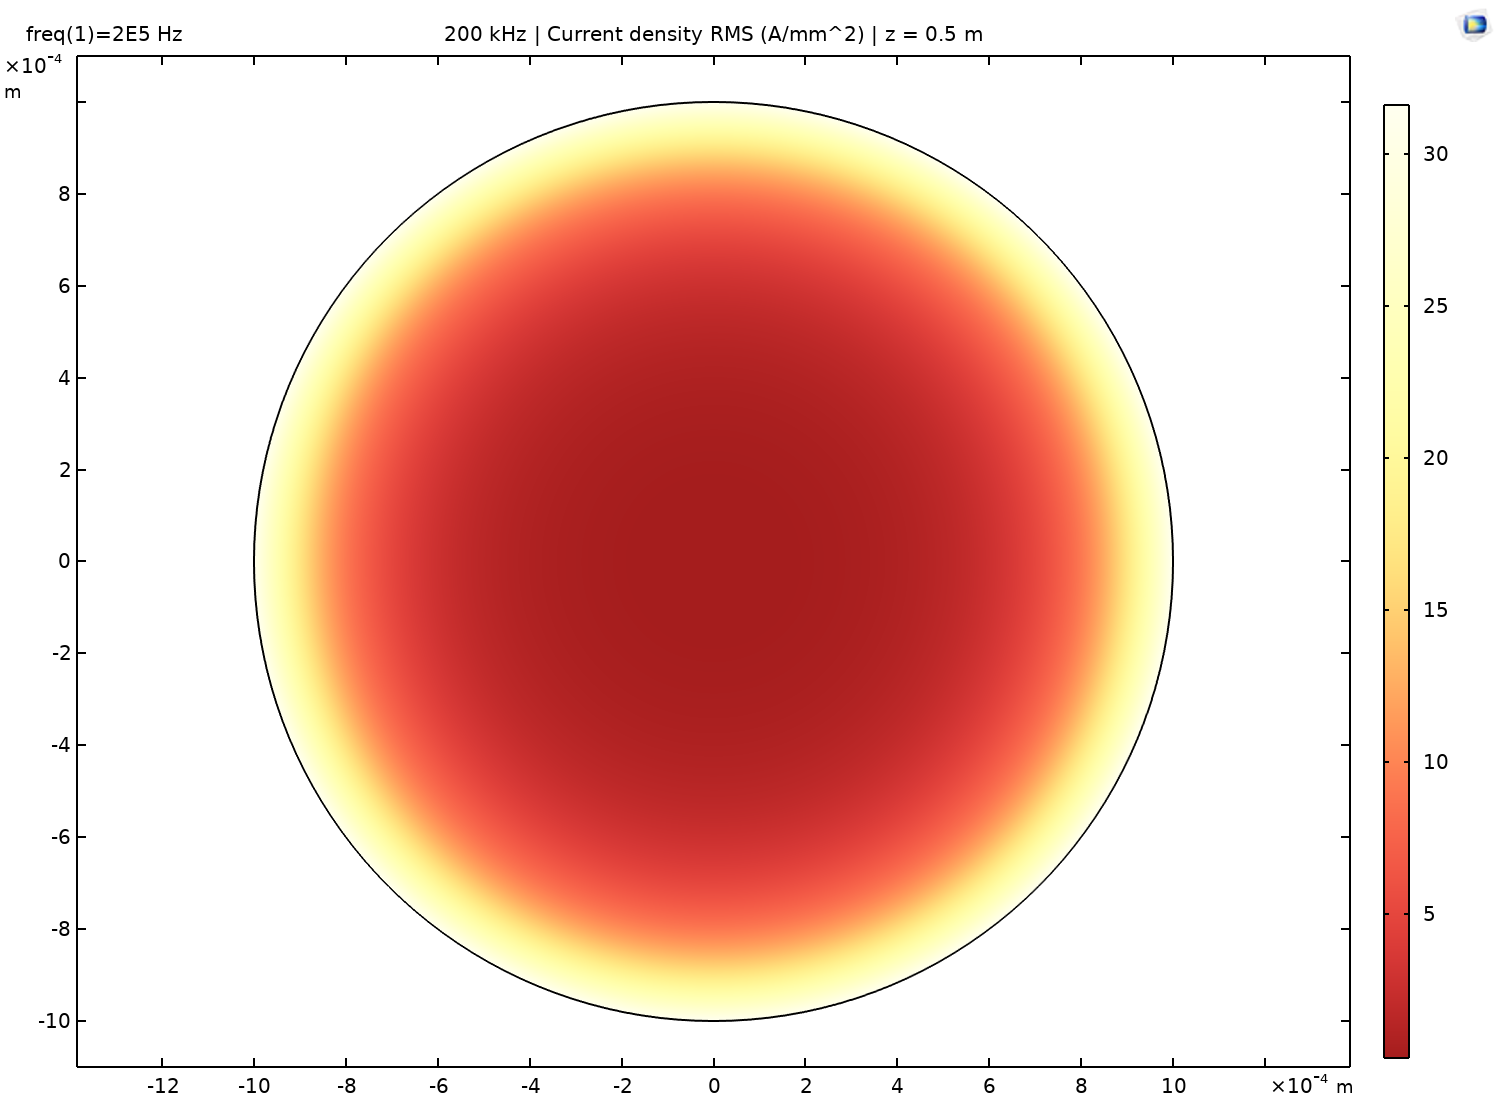
\includegraphics[width=0.62\textwidth]{figs/native_q1_cross_section.png}
\caption{实心铜导线横截面的电流密度有效值分布（COMSOL 原生导出）。
电流被强烈挤压至表面约 $\delta$ 厚的薄层内，轴心区域几乎不承担电流。}
\label{fig:q1-cross}
\end{figure}

图 \ref{fig:q1-cross} 直观呈现了趋肤效应：电流密度在表面处达
$31.60\U{A/mm^2}$，而轴心处仅 $0.279\U{A/mm^2}$，
两者相差约 \textbf{113 倍}。这意味着直径 $2\U{mm}$ 的实心铜线在
$200\U{kHz}$ 下，中心区域绝大部分铜材实际上处于「闲置」状态。

\subsubsection{径向电流密度分布}

图 \ref{fig:q1-radial} 给出沿半径的电流密度分布，并与圆柱导体的 Bessel 函数
精确解逐点对照。

\begin{figure}[H]
\centering
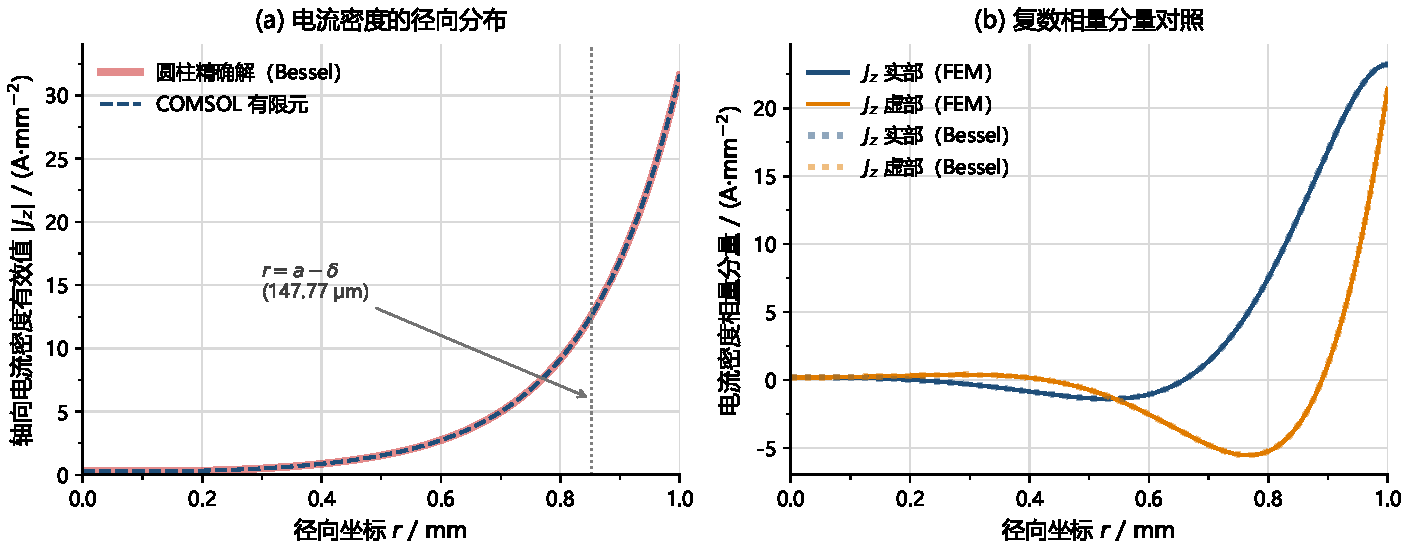
\includegraphics[width=\textwidth]{figs/q1_radial_J.pdf}
\caption{电流密度的径向分布。(a) 轴向电流密度有效值 $|J_z(r)|$：
有限元结果与 Bessel 精确解几乎完全重合；点线标出 $r = a-\delta$ 位置。
(b) 复数相量分量的逐点对照：实部与虚部均与解析解一致，
证实有限元解在相位上也是正确的。}
\label{fig:q1-radial}
\end{figure}

由图 \ref{fig:q1-radial} 可见，电流密度从轴心向外单调增大，
在表面附近达到峰值后（因表面为电流的「出口」）保持高位，
呈现典型的趋肤分布形貌。有限元曲线与解析解曲线在全部 2001 个径向采样点上
几乎完全重合，\textbf{最大绝对误差（归一化到表面幅值）仅 $0.0394\%$}。
图 \ref{fig:q1-radial}(b) 进一步表明，实部与虚部两个相量分量都吻合良好，
说明模型不仅复现了幅值衰减，也正确复现了电流的相位滞后。

\subsection{网格收敛性分析}
\label{sec:q1-mesh}

赛题明确要求给出网格收敛性说明。本文以径向单元数为变量做五档加密，
每档均独立求解，结果列于表 \ref{tab:q1-mesh}，图 \ref{fig:q1-mesh} 给出其可视化。

\begin{table}[H]
\centering
\caption{问题一：径向网格收敛性（五档独立求解）}
\label{tab:q1-mesh}
\small
\begin{adjustbox}{max width=\textwidth}
\begin{tabular}{c c c c c}
\toprule
\textbf{径向单元数} & \textbf{径向步长} & \textbf{四边形单元数} & $\Rac$ & \textbf{相对解析解误差} \\
 & $/\U{\mu m}$ & & $/\Umohm$ & $/\%$ \\
\midrule
8   & 125.0000 & 32  & 19.996449734 & $9.8689514\times10^{-2}$ \\
16  & 62.5000  & 64  & 20.015105571 & $5.4858388\times10^{-3}$ \\
32  & 31.2500  & 128 & 20.016137436 & $3.3069222\times10^{-4}$ \\
64  & 15.6250  & 256 & 20.016199530 & $2.0472846\times10^{-5}$ \\
\textbf{128} & \textbf{7.8125} & \textbf{512} & \textbf{20.016203372} & $\mathbf{1.2764727\times10^{-6}}$ \\
\bottomrule
\end{tabular}
\end{adjustbox}
\end{table}

\begin{figure}[H]
\centering
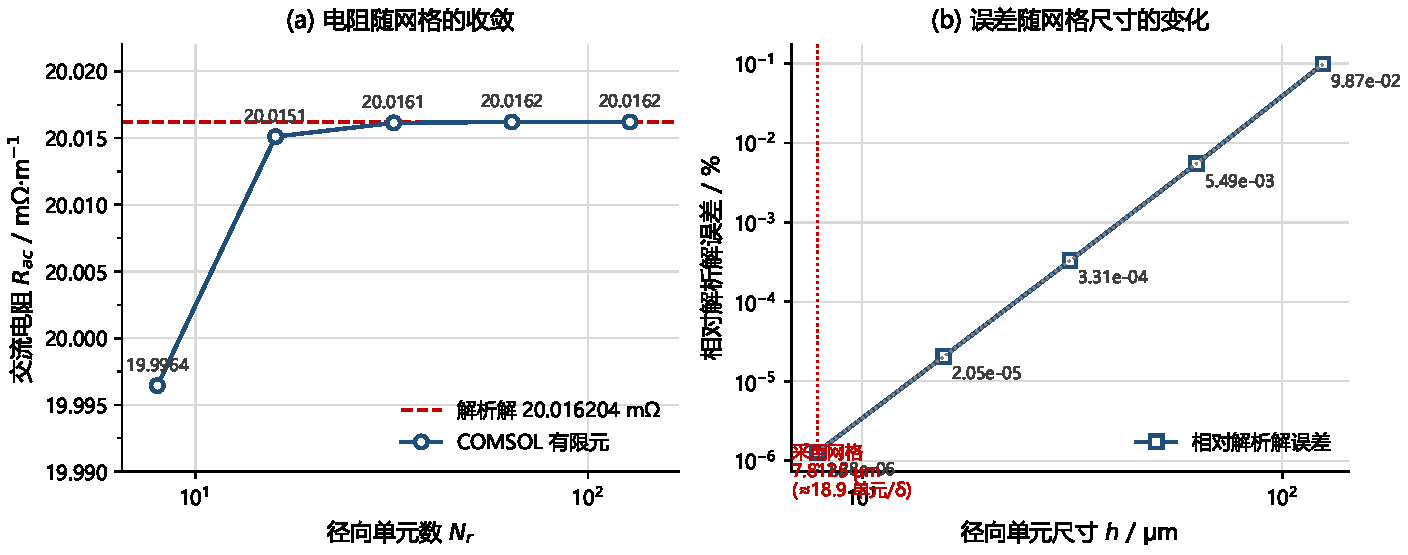
\includegraphics[width=\textwidth]{figs/q1_mesh_convergence.pdf}
\caption{网格收敛性分析。(a) $\Rac$ 随径向单元数的收敛过程，
虚线为 Bessel 精确解 $20.016204\Umohm$；
(b) 相对解析解误差随径向单元尺寸 $h$ 的变化（双对数坐标），
误差随 $h$ 减小呈单调下降，最终达到 $10^{-6}\%$ 量级。}
\label{fig:q1-mesh}
\end{figure}

\textbf{收敛性结论}：

\begin{enumerate}[label=(\arabic*), leftmargin=2.2em, itemsep=3pt]
\item $\Rac$ 随网格加密\textbf{单调收敛}，无振荡，说明离散格式稳定。
\item 最后两档网格（64 与 128）的 $\Rac$ 相对变化仅
$1.92\times10^{-5}\%$，最终档相对解析解误差为 $1.28\times10^{-6}\%$，
已达到双精度求解器的数值噪声水平，可认为\textbf{网格已完全收敛}。
\item \textbf{粗网格会低估损耗}：8 个径向单元时步长 $125\U{\mu m}$，
仅约 $1.18$ 个单元/$\delta$，$\Rac$ 被低估 $0.099\%$；
因为粗网格无法解析表层的陡峭梯度，梯度场被平滑后铜损偏低。
这提示\textbf{网格必须按趋肤深度而非按几何尺寸剖分}——本文最终采用
$18.9$ 单元/$\delta$，是一个有充分余量的选择。
\item 轴向网格的影响可以忽略：轴向单元由 4 增为 8 后，$\Rac$ 变化低于
$10^{-9}\%$。这符合物理直觉——电流沿轴向均匀，$z$ 方向无梯度，
轴向不需要与径向同等细化。
\item 需要强调，以上收敛性仅针对\textbf{本基准模型}的离散误差，
不包含材料参数不确定度、实际接线与端部效应等未建模因素。
\end{enumerate}

\subsection{与理论趋肤深度的交叉验证}
\label{sec:q1-verify}

\subsubsection{圆柱导体的精确解}

对半径 $a$ 的圆柱导体，磁扩散方程 \eqref{eq:diffusion} 的严格解由第一类 Bessel
函数给出。令 $k = (1-j)/\delta$，在有效值相量约定下

\begin{equation}
J_z(r) = \frac{I_{\mathrm{rms}}\,k}{2\pi a}\cdot\frac{J_0(kr)}{J_1(ka)},
\qquad
Z_{\mathrm{int}} = \frac{L\,k}{2\pi a\sigma}\cdot\frac{J_0(ka)}{J_1(ka)},
\qquad
\Rac = \operatorname{Re} Z_{\mathrm{int}} .
\label{eq:bessel}
\end{equation}

式 \eqref{eq:bessel} 仅用于\textbf{独立验证}有限元结果，不参与建模。
代入本题参数得解析电阻 $20.016203628\Uohm$，
与有限元的 $20.016203372\Uohm$ 相对误差 $1.28\times10^{-6}\%$，
两者在数值上等价。

\subsubsection{电流集中层厚度的定义与测量}

赛题问「仿真得到的电流集中层厚度与理论趋肤深度是否一致」。
平面波的 $1/e$ 判据不能直接照搬到圆柱导体上，因为圆柱的电流分布是 Bessel 型
而非指数型。为做同口径比较，本文统一采用
\textbf{$1/e$ 衰减层厚度}：由 $|J(a-t)|/|J(a)| = 1/e$ 反解 $t$。
结果列于表 \ref{tab:q1-skin}。

\begin{table}[H]
\centering
\caption{电流集中层厚度的三种口径对比}
\label{tab:q1-skin}
\small
\begin{adjustbox}{max width=\textwidth}
\begin{tabular}{l c l}
\toprule
\textbf{口径} & \textbf{厚度} $/\U{\mu m}$ & \textbf{说明} \\
\midrule
平面波趋肤深度 $\delta$（理论）        & 147.772 & 式 \eqref{eq:delta-value}，半无限平面导体 \\
圆柱 $1/e$ 衰减层（有限元）            & 160.983 & 由 COMSOL 径向场反解 \\
圆柱 $1/e$ 衰减层（Bessel 精确解）     & 160.994 & 由式 \eqref{eq:bessel} 反解 \\
\midrule
圆柱口径相对平面口径的偏差             & $+8.94\%$ & 曲率效应 \\
有限元与精确解之间的偏差               & $0.011\U{\mu m}$（$0.007\%$） & 数值误差可忽略 \\
\bottomrule
\end{tabular}
\end{adjustbox}
\end{table}

\textbf{结论}：仿真得到的电流集中层厚度 $160.983\U{\mu m}$ 与圆柱精确解
$160.994\U{\mu m}$ 相差仅 $0.011\U{\mu m}$，可以认为\textbf{有限元完全复现了
圆柱导体的电流分布规律}。它与平面波 $\delta = 147.772\U{\mu m}$ 相差 $8.94\%$，
这一偏差并非仿真错误，而是\textbf{曲率效应}的必然结果：
本题 $a/\delta \approx 6.77$，导体的曲率半径与趋肤深度之比不够大，
电流在圆柱内除了向表面集中外，还受到柱面弯曲的「额外聚焦」，
使衰减层比平面情形更厚。只有当 $a \gg \delta$ 时，圆柱的衰减层厚度才趋于平面 $\delta$。
\textbf{因此不能要求圆柱的 $1/e$ 厚度严格等于平面 $\delta$，两者相差 $9\%$ 属于合理范围。}

\subsection{频率扫描}

赛题鼓励在 $50\U{kHz}$--$1\U{MHz}$ 内做频率扫描分析。本文以最终网格
实际求解了七个频点，每个频点均为 $20\U{A}$ 有效值，结果列于表 \ref{tab:q1-freq}，
并与解析解逐点对照。

\begin{table}[H]
\centering
\caption{问题一：频率扫描结果（$50\U{kHz}$--$1\U{MHz}$，均为 $20\U{A}$ 有效值）}
\label{tab:q1-freq}
\small
\begin{adjustbox}{max width=\textwidth}
\begin{tabular}{c c c c c c}
\toprule
$f/\U{kHz}$ & $\delta/\U{\mu m}$ & $\Rac/\Umohm$ & $\Rac/\Rdc$ &
$P/\U{W/m}$ & \textbf{相对解析解误差}/$\%$ \\
\midrule
50   & 295.543 & 10.789453 & 1.965972 & 4.315781  & $-4.72\times10^{-8}$ \\
100  & 208.981 & 14.607310 & 2.661633 & 5.842924  & $-2.57\times10^{-7}$ \\
\textbf{200}  & \textbf{147.772} & \textbf{20.016203} & \textbf{3.647200} & \textbf{8.006481}  & $-1.28\times10^{-6}$ \\
300  & 120.655 & 24.176313 & 4.405223 & 9.670525  & $-3.17\times10^{-6}$ \\
500  & 93.459  & 30.780795 & 5.608642 & 12.312318 & $-9.73\times10^{-6}$ \\
750  & 76.309  & 37.370855 & 6.809432 & 14.948342 & $-2.33\times10^{-5}$ \\
1000 & 66.085  & 42.928639 & 7.822129 & 17.171456 & $-4.30\times10^{-5}$ \\
\bottomrule
\end{tabular}
\end{adjustbox}
\end{table}

\begin{figure}[H]
\centering
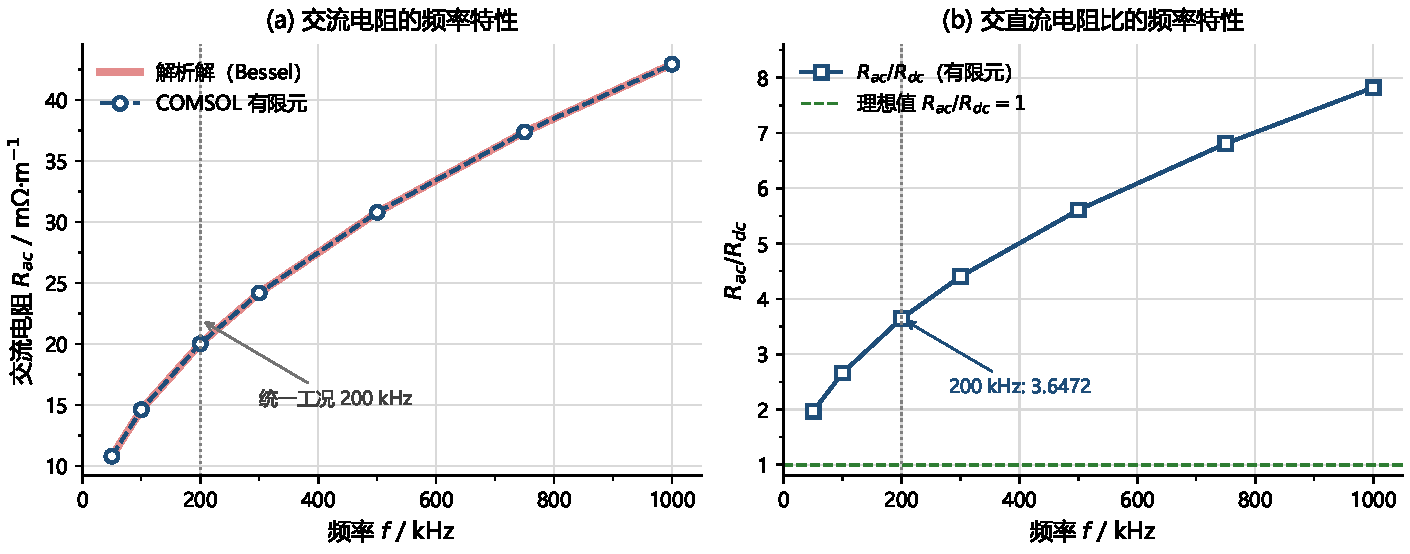
\includegraphics[width=\textwidth]{figs/q1_frequency_sweep.pdf}
\caption{实心导线的频率特性。(a) $\Rac$ 随频率的上升，
有限元与 Bessel 解析解在所有频点重合；
(b) $\Rac/\Rdc$ 随频率的上升，虚线为理想值 1。
$200\U{kHz}$ 处 $\Rac/\Rdc = 3.6472$。}
\label{fig:q1-freq}
\end{figure}

\begin{figure}[H]
\centering
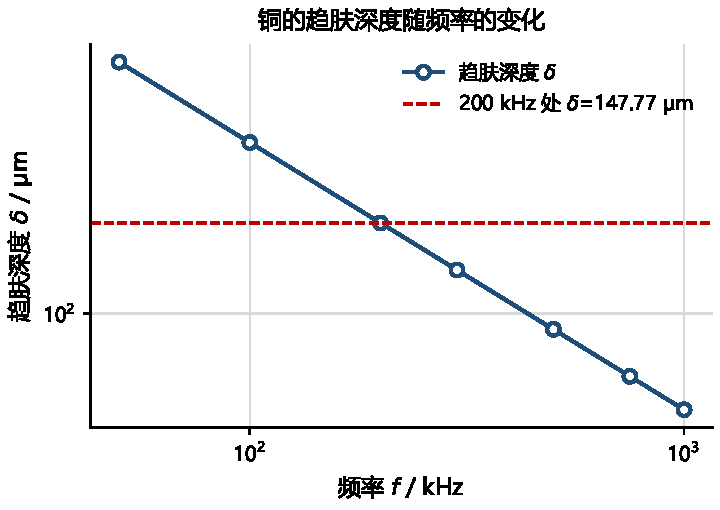
\includegraphics[width=0.56\textwidth]{figs/q1_skin_depth.pdf}
\caption{铜的趋肤深度随频率的变化（$\delta \propto f^{-1/2}$），
虚线标出统一工况 $200\U{kHz}$ 处的 $\delta = 147.77\U{\mu m}$。}
\label{fig:q1-skin}
\end{figure}

扫描结果表明：全部七个频点的有限元电阻与解析解最大相对误差为
$4.30\times10^{-5}\%$，误差随频率升高缓慢增大（因 $\delta$ 减小后
相对网格尺寸变大），但仍处于可忽略量级。
从物理趋势看，$\Rac$ 随 $f$ 近似按 $f^{1/2}$ 增长（$\delta \propto f^{-1/2}$
而有效导电截面 $\propto \delta$），$\Rac/\Rdc$ 从 $50\U{kHz}$ 的 $1.97$
单调升至 $1\U{MHz}$ 的 $7.82$。这说明\textbf{频率越高，
实心导线的损耗惩罚越严重，Litz 化的收益也越大}。

\subsection{关于题目条件的一处冲突}

本文在建模过程中发现统一工况中存在一处需要说明的冲突：
$\varnothing 2\U{mm}$ 导线的截面积为 $\pi\U{mm^2}\approx 3.1416\U{mm^2}$，
在 $20\U{A}$ 下对应 $J_{dc} = 6.3662\U{A/mm^2}$，
\textbf{超过了统一工况规定的 $4\U{A/mm^2}$ 温升约束}。

本文的处理方式是：\textbf{问题一保留赛题明确指定的直径 $2\U{mm}$ 与电流 $20\U{A}$}，
因为本题的目的是「走通流程并用理论交叉验证趋肤效应」，
而非满足温升约束；同时在该处显式指出冲突，避免误用。
相应地，问题二中做「等铜截面对照」时\textbf{不能}用问题一的 $2\U{mm}$ 导线，
而应改用与 Litz 线总铜截面相同的实心线
（$A = 5.0953\U{mm^2}$，等效直径 $2.5471\U{mm}$），详见 \S\ref{sec:q2-compare}。

\subsection{问题一小结}

问题一完整走通了「几何建模 $\to$ 材料与物理场设置 $\to$ 激励与边界 $\to$ 网格剖分 $\to$
频域求解 $\to$ 后处理提取 $\to$ 网格收敛 $\to$ 解析交叉验证」的全流程，
所有结论均由本机 COMSOL 6.2 的真实有限元求解支撑。核心数据为：

\begin{equation*}
\Rac = 20.0162\Uohm,\quad
\Rac/\Rdc = 3.6472,\quad
P = 8.0065\U{W/m},\quad
\delta = 147.772\U{\mu m}.
\end{equation*}

该结果同时揭示了一个关键的工程事实：\textbf{在 $200\U{kHz}$ 下，
一根 $2\U{mm}$ 实心铜线的交流电阻是其直流电阻的 $3.65$ 倍，
其中绝大部分铜材（轴心区域）处于闲置状态}。
这正是问题二引入 Litz 线的直接动因。

% =====================================================================
%  四、问题二
% =====================================================================
\section{问题二：Litz 线的设计与仿真}

\subsection{设计约束与参数确定}

\subsubsection{丝径判据：为什么是 $d = 0.14\U{mm}$}

丝径的选择依据是\textbf{丝径系数} $\beta = d/\delta$。只要 $\beta < 1$，
单丝内部的趋肤效应就可忽略；但 $\beta$ 也不是越小越好——
丝越细，绝缘占比与加工成本越高，且同样铜截面下股数 $N$ 急剧增加
（$N \propto 1/d^2$），制造难度与丝间邻近效应耦合的复杂度同步上升。

本文取

\begin{equation}
\beta = \frac{d}{\delta} = \frac{0.14\U{mm}}{0.147772\U{mm}} = 0.9474 < 1 .
\label{eq:beta}
\end{equation}

该取值使单丝直径略小于趋肤深度，在「单丝趋肤效应基本消除」与
「股数不过多、绝缘占比不过高」之间取得平衡。作为对照，
孤立的 $0.14\U{mm}$ 铜丝在 $200\U{kHz}$ 下的理论
$\Rac/\Rdc$ 仅为 $1.00105$（由 \texttt{results\_summary.json} 中的
\texttt{isolated\_strand\_Rac\_Rdc\_theory} 给出），
即\textbf{单丝内部的趋肤损耗几乎可以忽略}——这验证了 $\beta < 1$ 判据的有效性，
也说明后续出现的全部额外损耗都来自\textbf{丝与丝之间的邻近效应}。

\subsubsection{股数与总铜截面：由温升约束确定}

由统一工况的 $J_{dc}\le 4\U{A/mm^2}$ 与 $I = 20\U{A}$，最小铜截面为

\begin{equation}
A_{\min} = \frac{I}{J_{dc}} = \frac{20\U{A}}{4\U{A/mm^2}} = 5\U{mm^2} .
\end{equation}

在 $d = 0.14\U{mm}$ 下，单丝截面积 $A_0 = \pi d^2/4 = 1.53938\times10^{-2}\U{mm^2}$，
故所需股数

\begin{equation}
N \ge \frac{A_{\min}}{A_0} = \frac{5}{0.0153938} \approx 324.8
\quad\Longrightarrow\quad N_{\min} = 325 .
\end{equation}

本文采用\textbf{同心圆环排布}：中心 1 股，外围 10 个同心圆环，第 $k$ 环放置 $6k$ 股，
环半径步长 $p = 0.15\U{mm}$，则

\begin{equation}
N = 1 + \sum_{k=1}^{10} 6k = 1 + 6\cdot\frac{10\times11}{2} = 331 .
\label{eq:N331}
\end{equation}

该排布同时满足三个条件：
\begin{enumerate}[label=(\alph*), leftmargin=2.2em, itemsep=2pt]
\item 股数 $331 \ge 325$，满足温升约束；
\item 采用完整 10 个圆环（而非截断到 325 股）使结构具有\textbf{六重旋转对称性}，
几何规整、便于参数化建模与后续编织拓扑的推广；
\item 相邻环半径差 $0.15\U{mm}$ 大于丝径 $0.14\U{mm}$，
同环内最近邻弦长亦不小于 $0.15\U{mm}$，
故\textbf{全模型铜表面最小间隙为 $10\U{\mu m}$}，丝间绝缘可制造。
\end{enumerate}

\subsubsection{设计参数汇总}

\begin{table}[H]
\centering
\caption{问题二：Litz 线设计参数}
\label{tab:q2-design}
\small
\begin{adjustbox}{max width=\textwidth}
\begin{tabular}{l l l}
\toprule
\textbf{参数} & \textbf{数值} & \textbf{依据} \\
\midrule
单股裸铜丝径 $d$            & $0.14\U{mm}$            & $\beta = d/\delta = 0.9474 < 1$ \\
股数 $N$                    & $331$                      & 满足 $N\ge325$，且构成完整 10 环 \\
排布方式                    & 中心 1 股 + 第 $k$ 环 $6k$ 股 & 六重旋转对称，几何规整 \\
环半径步长 $p$              & $0.15\U{mm}$            & 保证丝间最小间隙 $10\U{\mu m}$ \\
最外层股心半径              & $1.50\U{mm}$            & $10p$ \\
裸铜束包络直径              & $3.14\U{mm}$            & 含漆膜后实际外径更大 \\
丝间最小铜表面间隙          & $10\U{\mu m}$           & 可制造性约束 \\
总铜截面 $A$                & $5.095349\U{mm^2}$      & $\ge 5\U{mm^2}$，满足温升约束 \\
直流平均电流密度 $J_{dc}$   & $3.925148\U{A/mm^2}$    & $< 4\U{A/mm^2}$，满足温升约束 \\
评估长度 $L$                & $1\U{m}$                & 统一工况 \\
\bottomrule
\end{tabular}
\end{adjustbox}
\end{table}

\subsection{几何建模}

\subsubsection{圆形简单成束（基线方案）}

第 $k$ 环第 $j$ 根股线的中心线为一条平行于 $z$ 轴的直线：

\begin{equation}
\bm\gamma_{k,j}(z) =
\left(kp\cos\frac{2\pi j}{6k},\ kp\sin\frac{2\pi j}{6k},\ z\right),
\qquad j = 0,1,\dots,6k-1,\quad 0\le z\le 1\U{m},
\label{eq:circular-geom}
\end{equation}

中心股单独置于 $(0,0,z)$。全部 331 根股线截面半径为 $0.07\U{mm}$。
该几何的\textbf{关键特征是所有股线沿全长保持固定的径向位置}——
这正是本文要考察的「未换位」基线。

\begin{figure}[H]
\centering
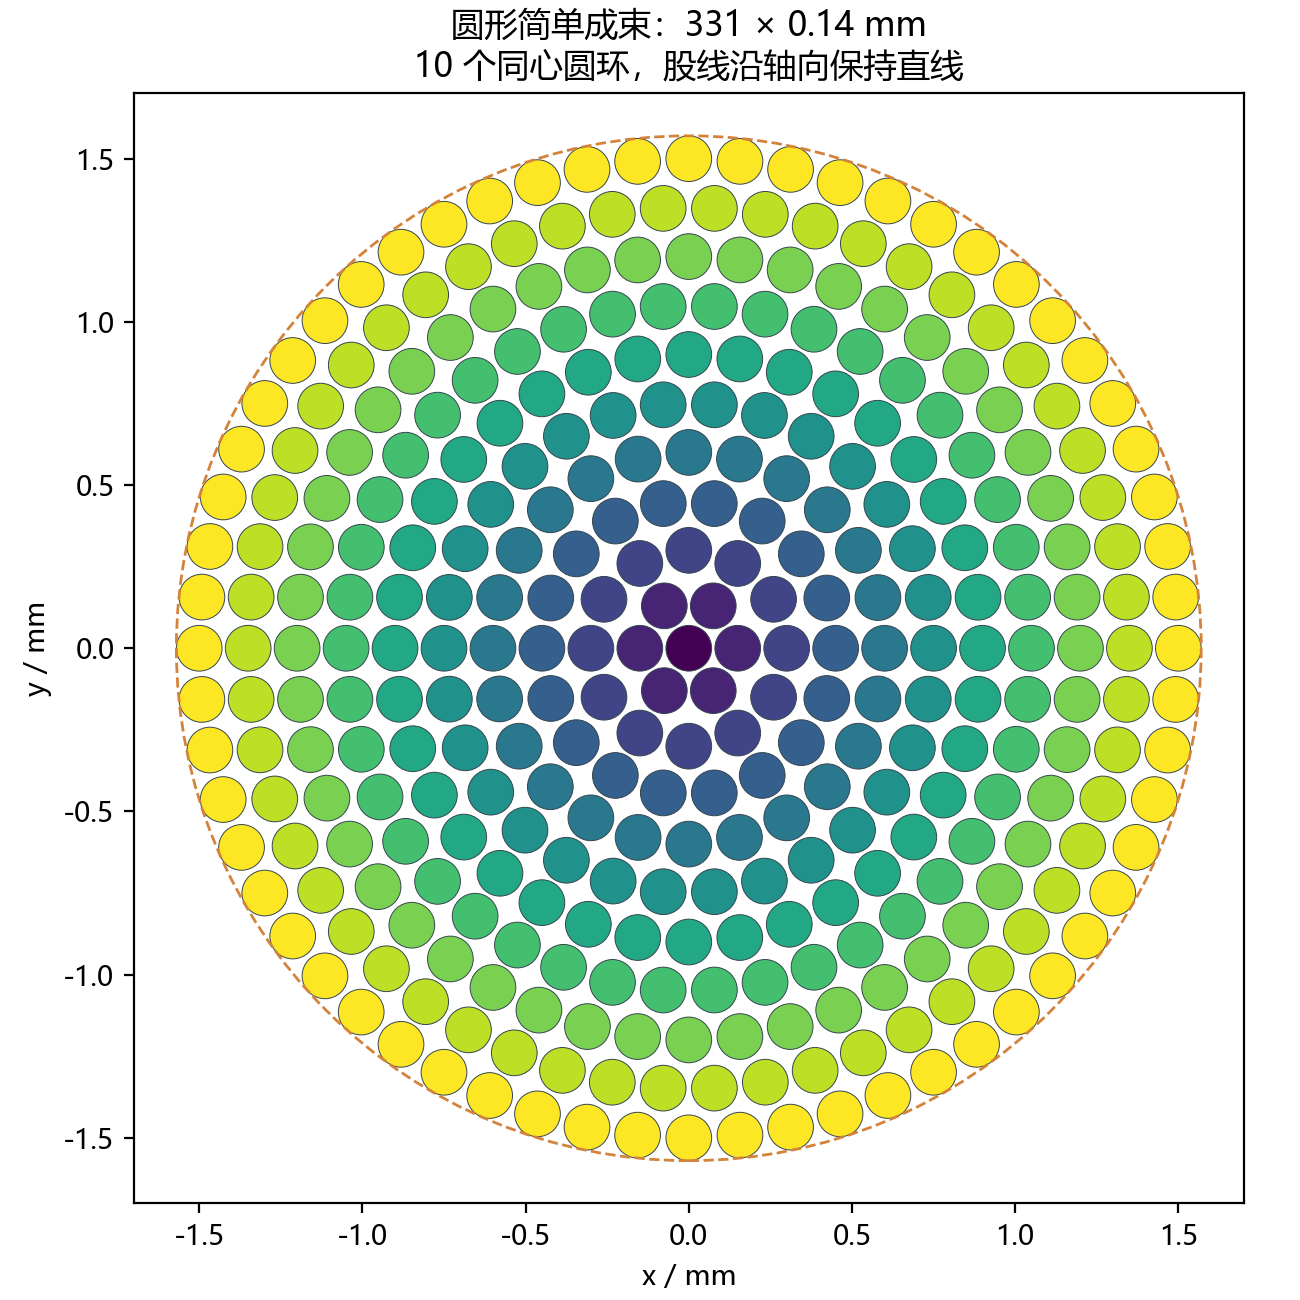
\includegraphics[width=0.60\textwidth]{figs/native_q2_layout.png}
\caption{圆形同心环排布的 331 股 Litz 线横截面。颜色仅区分圆环编号，
不代表电流大小。该方案具有六重旋转对称性。}
\label{fig:q2-layout}
\end{figure}

\begin{figure}[H]
\centering
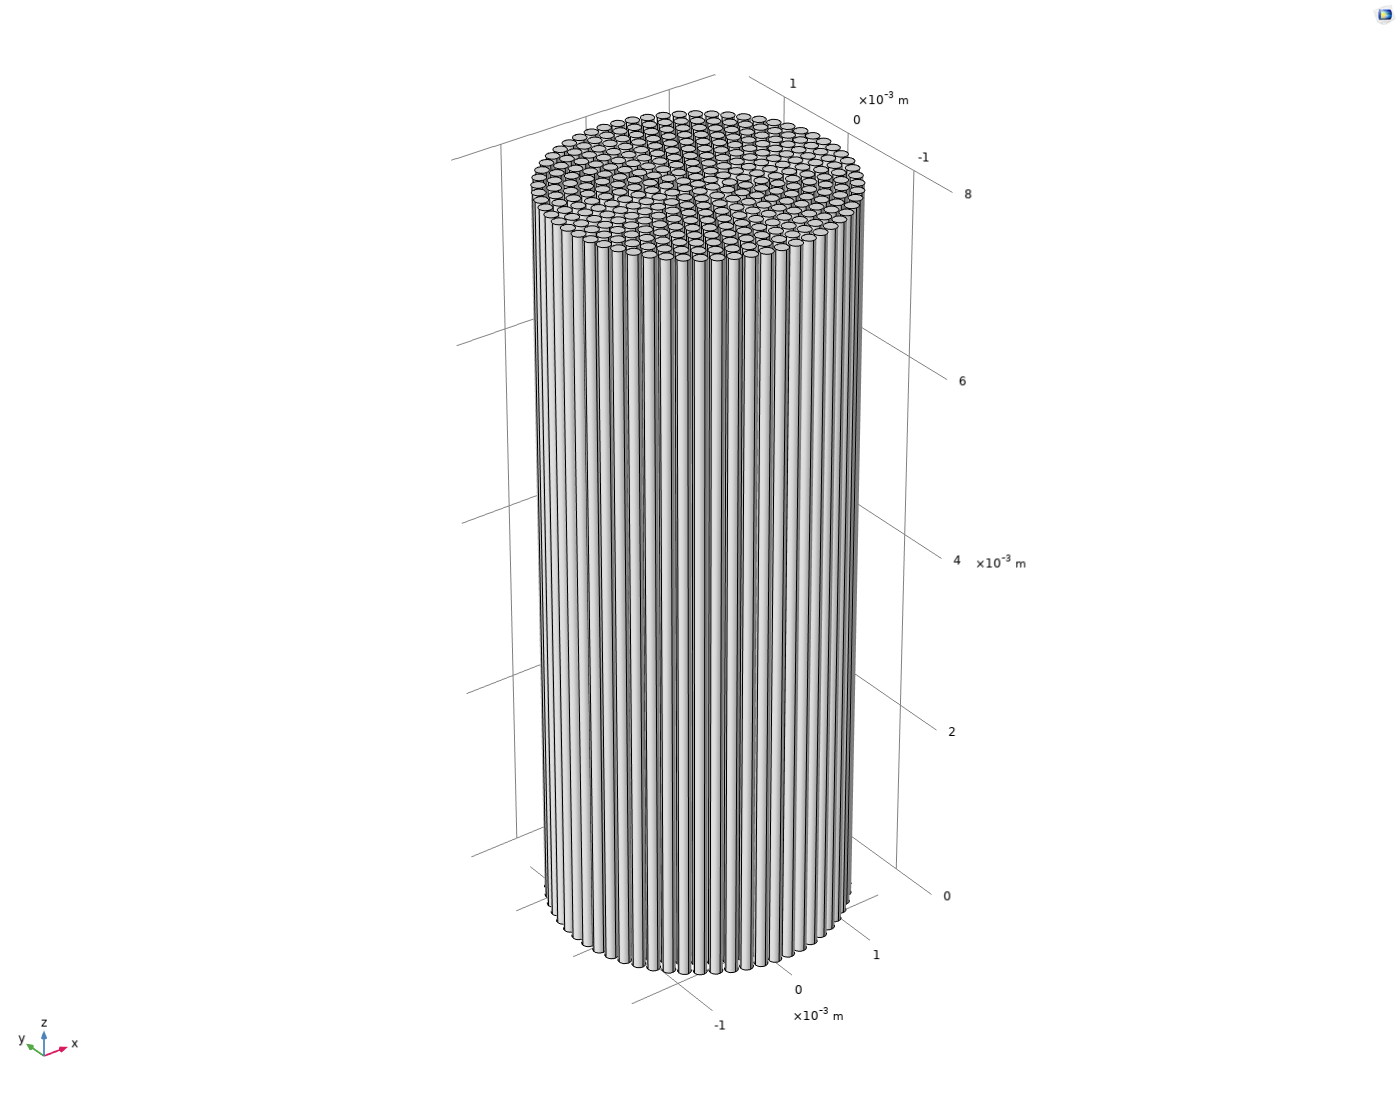
\includegraphics[width=0.56\textwidth]{figs/native_q2_3d_excerpt.png}
\caption{完整 $1\unit{m}$ 三维几何中的 331 根独立铜圆柱（COMSOL 预览仅显示
$8\unit{mm}$ 展示截段，以便辨认股线；保存的三维工程仍为完整 $1\unit{m}$）。
该几何由参数化脚本生成，可随 $d$、$N$、$p$ 等参数自动重建。}
\label{fig:q2-3d}
\end{figure}

\subsubsection{规则绞合方案（结构改进）}

为考察「传统绞合」这一最常用的换位手段的实际效果，
本文在同一股数、同一丝径、同一铜截面的前提下，
建立绞距 $P_{\mathrm{twist}} = 40\U{mm}$ 的规则绞合模型。
第 $k$ 层第 $j$ 股的中心线为等半径螺旋：

\begin{equation}\small
\mathbf c_{kj}(z) =
\left[r_k\cos(\theta_{kj}+\alpha z),\ r_k\sin(\theta_{kj}+\alpha z),\ z\right],
\qquad
r_k = 0.15k\U{mm},\quad
\theta_{kj} = \frac{2\pi j}{6k},\quad
\alpha = \frac{2\pi}{P_{\mathrm{twist}}} .
\label{eq:twist-geom}
\end{equation}

代入 $P_{\mathrm{twist}} = 40\U{mm}$ 得绞率 $\alpha = 157.080\U{1/m}$，
每轴向米 25 圈，最外层螺旋角 $13.258^\circ$。

\textbf{这里必须指出绞合的几何本质}：式 \eqref{eq:twist-geom} 中
$r_k$ 是\textbf{常数}，即每股的径向层号 $k$ 沿全长不变，
只有方位角 $\theta$ 在变化。因此\textbf{外层丝永远在外层，
只是换了一个角度，从未真正进入过内层}——绞合提供的换位是不彻底的。
这一点在 \S\ref{sec:q2-twist} 的结果中得到数据证实。

\begin{figure}[H]
\centering
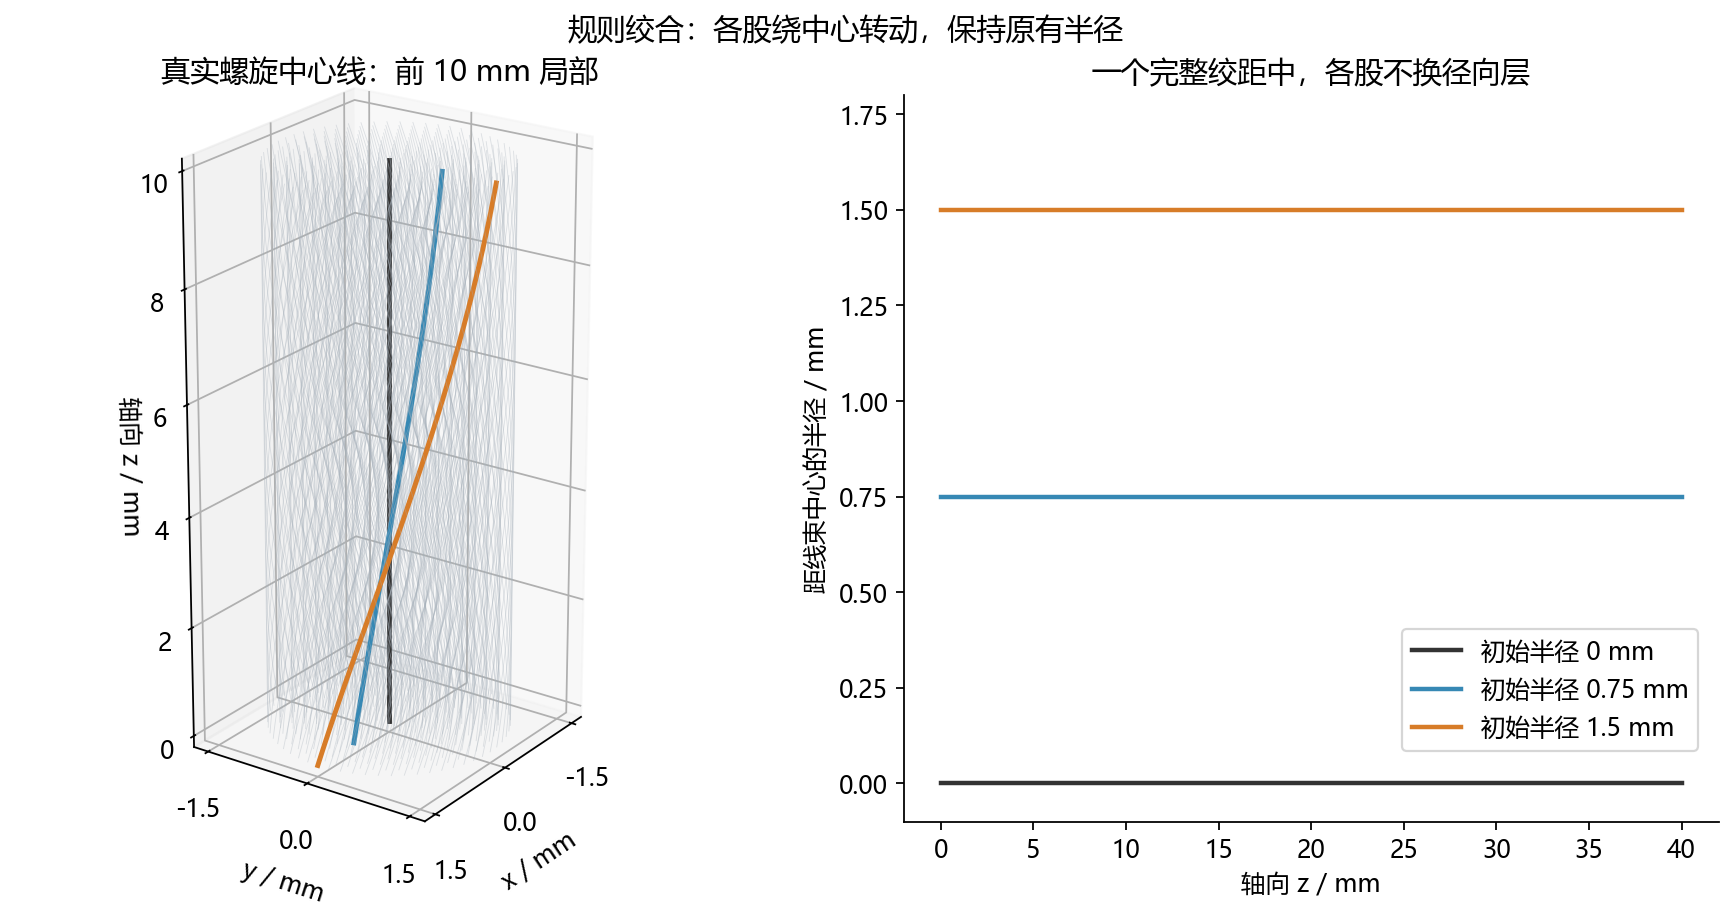
\includegraphics[width=0.86\textwidth]{figs/native_q2_twist_geometry.png}
\caption{规则绞合方案的中心线与径向层示意。各层半径恒定，
股线只做等半径螺旋运动，径向位置不随 $z$ 改变。}
\label{fig:q2-twist-geom}
\end{figure}

\begin{figure}[H]
\centering
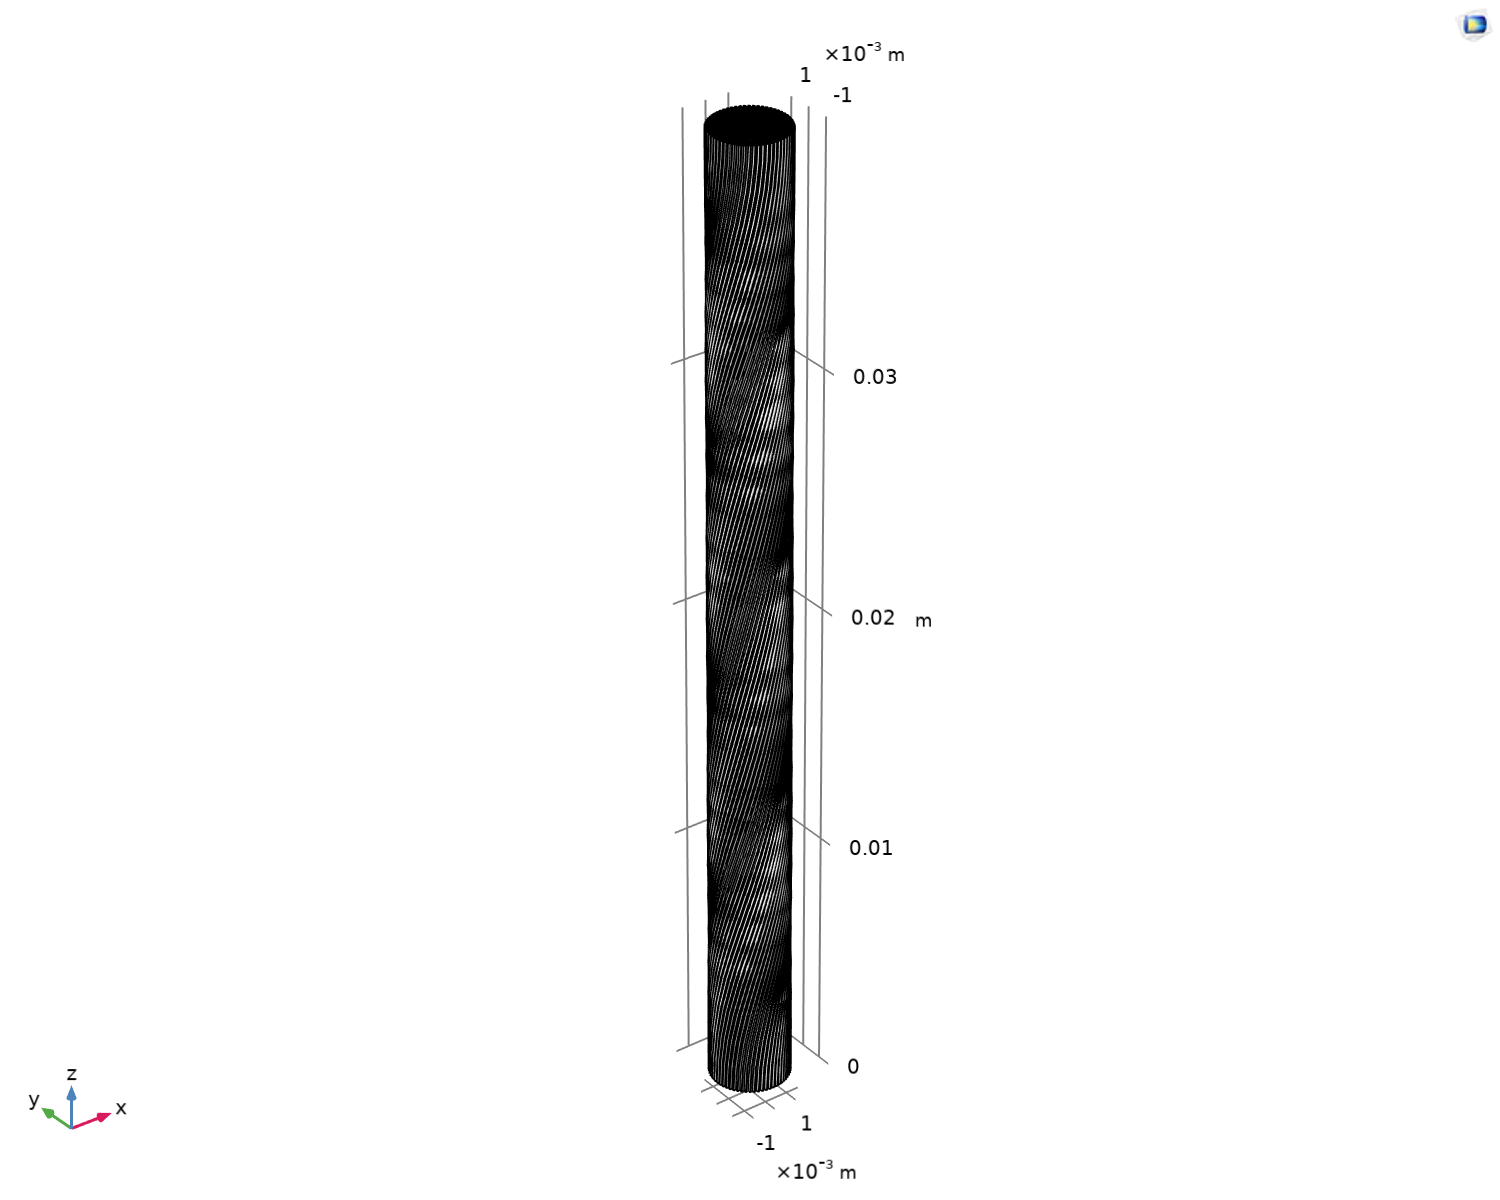
\includegraphics[width=0.52\textwidth]{figs/native_q2_twist_3d.png}
\caption{规则绞合的 331 根真实螺旋铜丝三维几何（一个 $40\U{mm}$ 绞距）。
本图仅用于结构展示；电磁计算采用螺旋坐标降维，见 \S\ref{sec:q2-solver}。}
\label{fig:q2-twist-3d}
\end{figure}

\subsubsection{绞合带来的几何代价}

绞合并非「免费」的改进：股线变成螺旋后实际长度增加。
由长度因子 $s_i = \sqrt{1+(\alpha r_i)^2}$，最外层每股每轴向米的实际线长为
$1.027383339\U{m}$，故每轴向米的铜体积由 $5.095349\U{cm^3}$
增至 $5.172137\U{cm^3}$，\textbf{增加 $1.507011\%$}。
相应地，$10\U{Hz}$ 校验下的最大电流密度为 $3.984012\U{A/mm^2}$，
仍小于 $4\U{A/mm^2}$ 约束，但已接近上限。

\subsection{电磁仿真设置}
\label{sec:q2-solver}

\subsubsection{圆形简单成束：二维截面磁矢势法}

由于 331 根直线股线沿 $z$ 方向不变，该结构是严格的二维问题。
采用 AC/DC 模块 \textbf{Magnetic Fields (\texttt{mf})} 接口，
求解面外磁矢势 $A_z$ 的频域方程。逐根保留 331 个独立铜域，
股间区域电导率设为 $0\U{S/m}$，相对磁导率取 1；
$10\U{\mu m}$ 的几何空隙等效表示丝间绝缘，
未单独建立漆膜的介电或热学模型。

\textbf{激励方式}：全部铜域由同一个 Single conductor Coil 节点激励
（Coil group 关闭），施加总电流峰值 $I_{\mathrm{pk}} = 20\sqrt{2}\U{A}$。
各股共用一个未知轴向电压梯度，通过积分约束维持总电流；
\textbf{每股电流由求解自然确定，没有施加任何强制均分}——
这是观察邻近效应所必需的条件。

外部非导电圆域半径取 $20\U{mm}$，边界采用磁绝缘 $A_z = 0$；
另用半径 $40\U{mm}$ 的模型检验边界截断影响。

主要积分关系为

\begin{equation}
\tilde I_i = \frac{1}{\sqrt2}\int_{\Omega_i} J_z\,\mathrm{d}A,
\qquad
P_i = L\int_{\Omega_i}\frac{|J_z|^2}{2\sigma}\,\mathrm{d}A,
\qquad
\Rac = \frac{\sum_i P_i}{I^2}.
\label{eq:q2-post}
\end{equation}

再次强调：总电流必须对\textbf{复相量}求和，各股电流幅值之和通常不等于 $20\U{A}$。

\subsubsection{规则绞合：螺旋坐标三分量降维}

绞合结构不再具有平移对称性，直接对 $1\U{m}$ 长的 331 根螺旋做完整三维有限元
计算量过大。本文利用结构的\textbf{螺旋对称性}，
在螺旋坐标变换下把问题降为二维三分量求解。

令参考截面 $z=0$ 上的映射 Jacobian 为

\begin{equation}
F = \begin{bmatrix}
1 & 0 & -\alpha y \\
0 & 1 & \alpha x \\
0 & 0 & 1
\end{bmatrix},
\qquad
K = F^{-1}F^{-T} =
\begin{bmatrix}
1+\alpha^2y^2 & -\alpha^2xy & \alpha y \\
-\alpha^2xy & 1+\alpha^2x^2 & -\alpha x \\
\alpha y & -\alpha x & 1
\end{bmatrix}.
\end{equation}

在铜域中取等效电导率 $\sigma' = \sigma K$，全部区域取 $\mu' = \mu K$，
绝缘区取 $\sigma' = 0$，求解 $A_x, A_y, A_z$ 三个分量。
公共电压梯度 $E_0$ 对应的源电流为
$\mathbf J'_{\mathrm{src}} = \sigma E_0[\alpha y, -\alpha x, 1]^{\mathsf T}$。
由变换空间电流恢复真实空间电流 $\mathbf J = F\mathbf J'$，再按式
\eqref{eq:q2-post} 提取损耗与电阻。该降维方法保留了周向电流分量、
真实线长与磁场耦合，其正确性由零绞度极限与低频极限两项校验确认
（见 \S\ref{sec:q2-verify}）。

\subsubsection{网格与求解}

两种方案均采用二阶单元。圆形方案铜域最大单元尺寸分别取 $d/3$、$d/5$、$d/8$
（对应 $46.667$、$28.0$、$17.5\U{\mu m}$），最小尺寸 $2.5\U{\mu m}$，
网格增长率 1.25，主模型采用 $d/8$ 档位。绞合方案采用相同口径的网格参数，
主模型自由度 660587，求解器为 GMRES + MUMPS 预条件，相对容差 $10^{-5}$，
丝间电导率严格保持 $0\U{S/m}$。

\subsection{结果与对比}
\label{sec:q2-compare}

\subsubsection{三方案等铜截面对照}

为保证可比性，所有方案均满足：总铜截面 $5.095349\U{mm^2}$、
$I = 20\U{A}$ 有效值、$f = 200\U{kHz}$、评估长度 $1\U{m}$。
对照结果列于表 \ref{tab:q2-compare}，可视化见图 \ref{fig:q2-compare}。

\begin{table}[H]
\centering
\caption{问题二：三种结构的等铜截面对照（$200\U{kHz}$，$20\U{A}$ 有效值）}
\label{tab:q2-compare}
\small
\begin{adjustbox}{max width=\textwidth}
\begin{tabular}{l c c c c}
\toprule
\textbf{结构} & $\Rdc$ & $\Rac$ & $\Rac/\Rdc$ & \textbf{每米铜损} \\
 & $/\Uohm$ & $/\Uohm$ & & $/\U{W/m}$ \\
\midrule
等铜截面实心圆线（$\varnothing 2.5471\U{mm}$） & 3.383748 & 15.463402 & 4.569903 & 6.185361 \\
六边形简单成束                                  & 3.383748 & 15.762611 & 4.658328 & 6.305045 \\
圆形简单成束（本文基线）                        & 3.383748 & \textbf{14.899678} & \textbf{4.403305} & \textbf{5.959871} \\
\midrule
规则绞合（绞距 $40\U{mm}$）                  & 3.434493 & \textbf{14.401182} & \textbf{4.193102} & \textbf{5.760473} \\
\bottomrule
\end{tabular}
\end{adjustbox}
\end{table}

\begin{figure}[H]
\centering
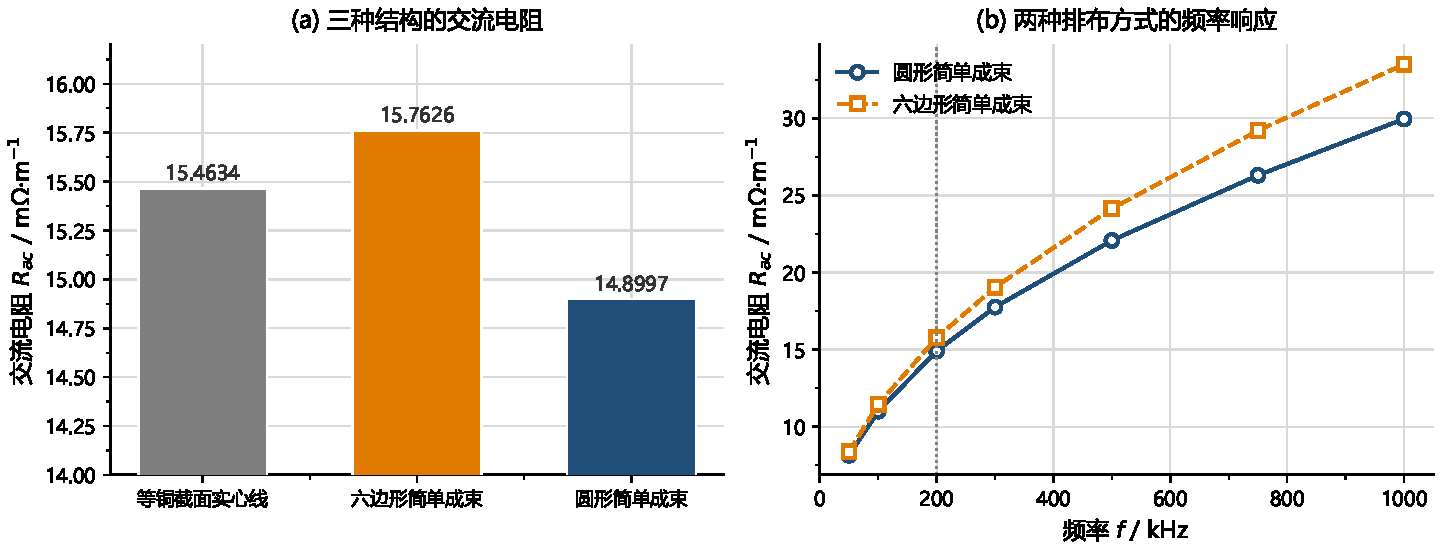
\includegraphics[width=\textwidth]{figs/q2_structure_compare.pdf}
\caption{(a) 三种等铜截面结构的交流电阻对照：圆形排布优于六边形排布；
(b) 两种排布方式的频率响应（$50\U{kHz}$--$1\U{MHz}$，均为真实 COMSOL 求解），
圆形排布在全频段均优于六边形。}
\label{fig:q2-compare}
\end{figure}

\subsubsection{关键观察}

\begin{enumerate}[label=(\arabic*), leftmargin=2.2em, itemsep=3pt]
\item \textbf{Litz 化带来明确收益，但远未达到理想}。
等铜截面实心线的 $\Rac/\Rdc = 4.5699$，圆形 Litz 束为 $4.4033$，
仅改善 $3.65\%$。若换位彻底、各股电流完全均分，
理论上的 $\Rac/\Rdc$ 应接近单丝的 $1.00105$。
\textbf{实际值与理想值之间存在巨大差距（$4.40$ vs $1.00$），
这 $3.4$ 倍的额外损耗就是邻近效应的代价。}
\item \textbf{排布方式本身有影响}。圆形排布相对六边形排布降低 $\Rac$ 达 $5.4746\%$。
需说明的是，圆形方案不仅改变了外轮廓，内部股线位置也随之变化，
因此该比较同时包含外轮廓与内部排布的影响，
\textbf{不应解释为「只改变外轮廓」这一单一参数的实验}。
\item \textbf{绞合进一步改善，但仍未解决根本问题}。
规则绞合相对圆形简单成束再降低 $3.3457\%$（$\Rac = 14.4012\Uohm$，
$\Rac/\Rdc = 4.1931$），相对等铜截面实心线降低 $6.8693\%$。
绞合改变了线长与电磁耦合，使部分邻近效应被平均掉；
但由于\textbf{径向层固定}（式 \eqref{eq:twist-geom}），
内层股线始终处于弱场、外层股线始终处于强场，损耗分摊依然极不公平
（详见 \S\ref{sec:q2-twist}）。\textbf{不能据一个绞距的结果断言已找到最优方案。}
\item \textbf{绞合存在几何代价}。绞合使每轴向米铜体积增加 $1.507\%$，
即用 $1.5\%$ 的额外铜材换取 $3.35\%$ 的损耗下降。
在等铜截面的严格约束下，这一代价需在问题三中纳入权衡。
\end{enumerate}

\begin{figure}[H]
\centering
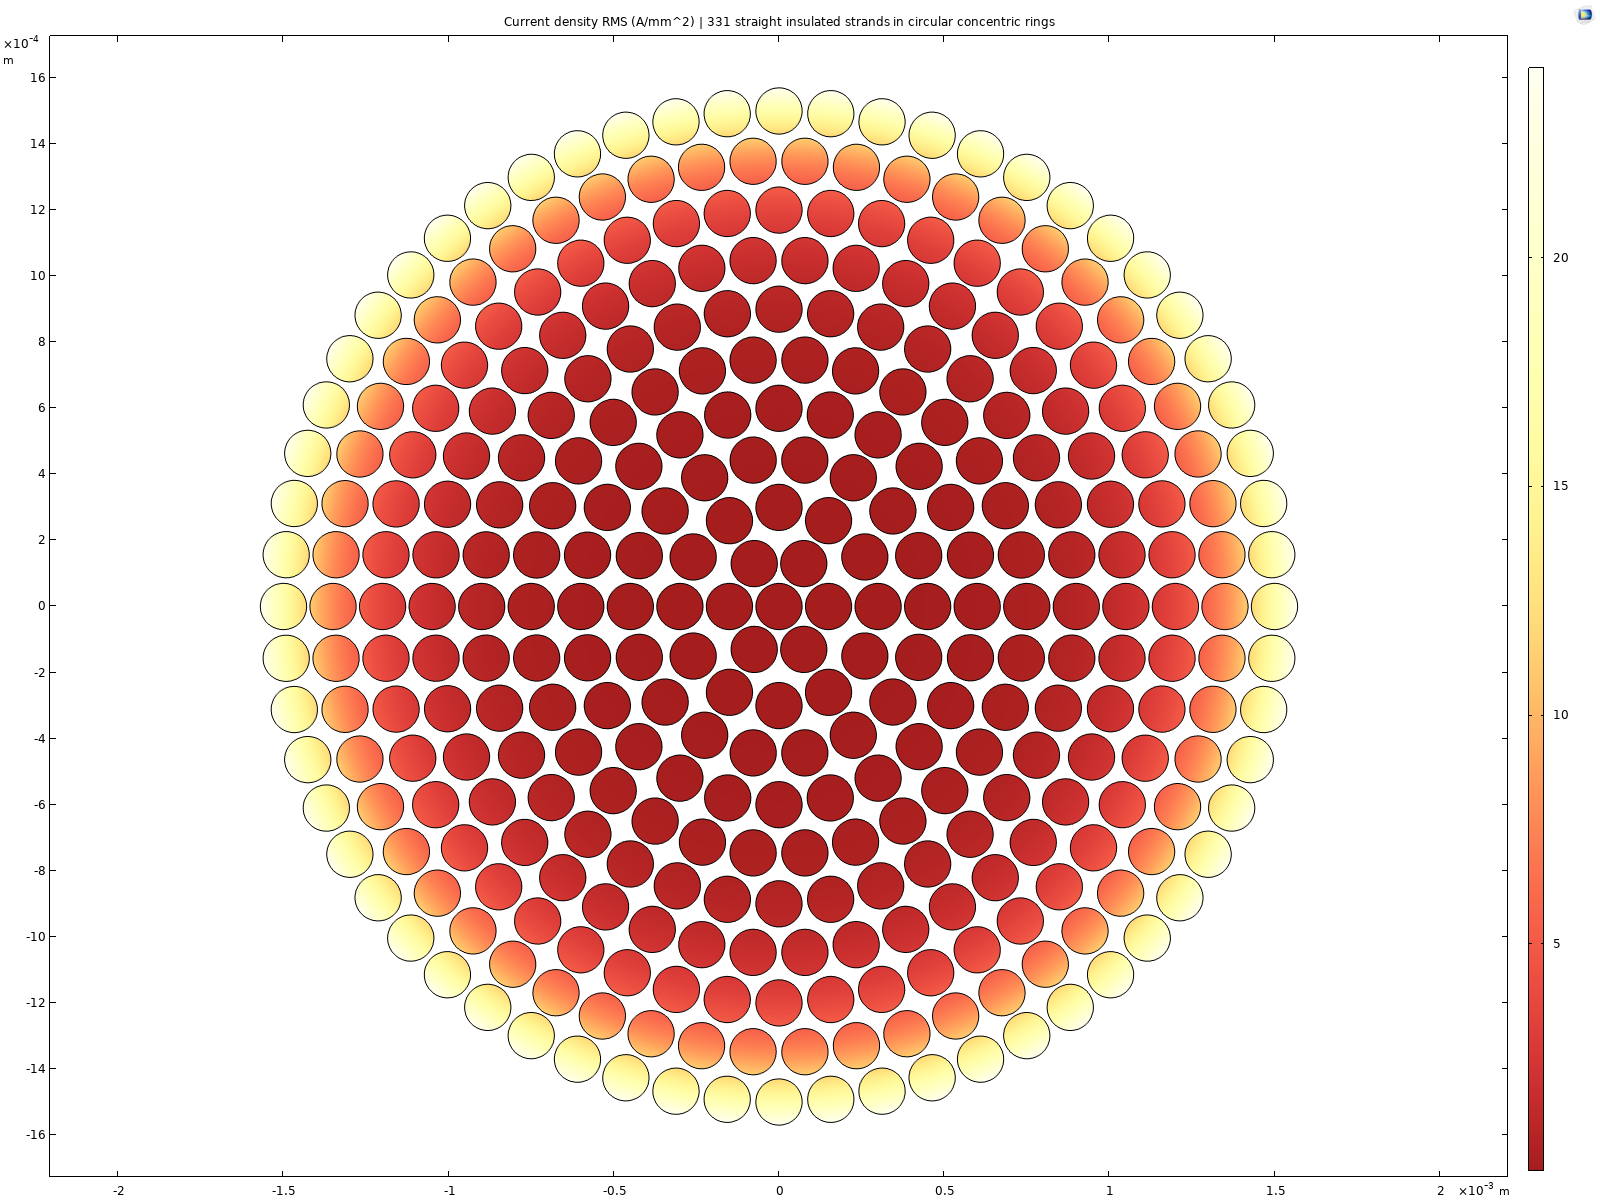
\includegraphics[width=0.92\textwidth]{figs/native_q2_current_density.png}
\caption{圆形简单成束中各股内部的局部电流密度有效值分布（COMSOL 原生云图）。
该云图包含单丝自身趋肤效应与丝间邻近效应的\textbf{共同}作用，
可见单丝内部电流本身也不均匀。}
\label{fig:q2-local-j}
\end{figure}

\begin{figure}[H]
\centering
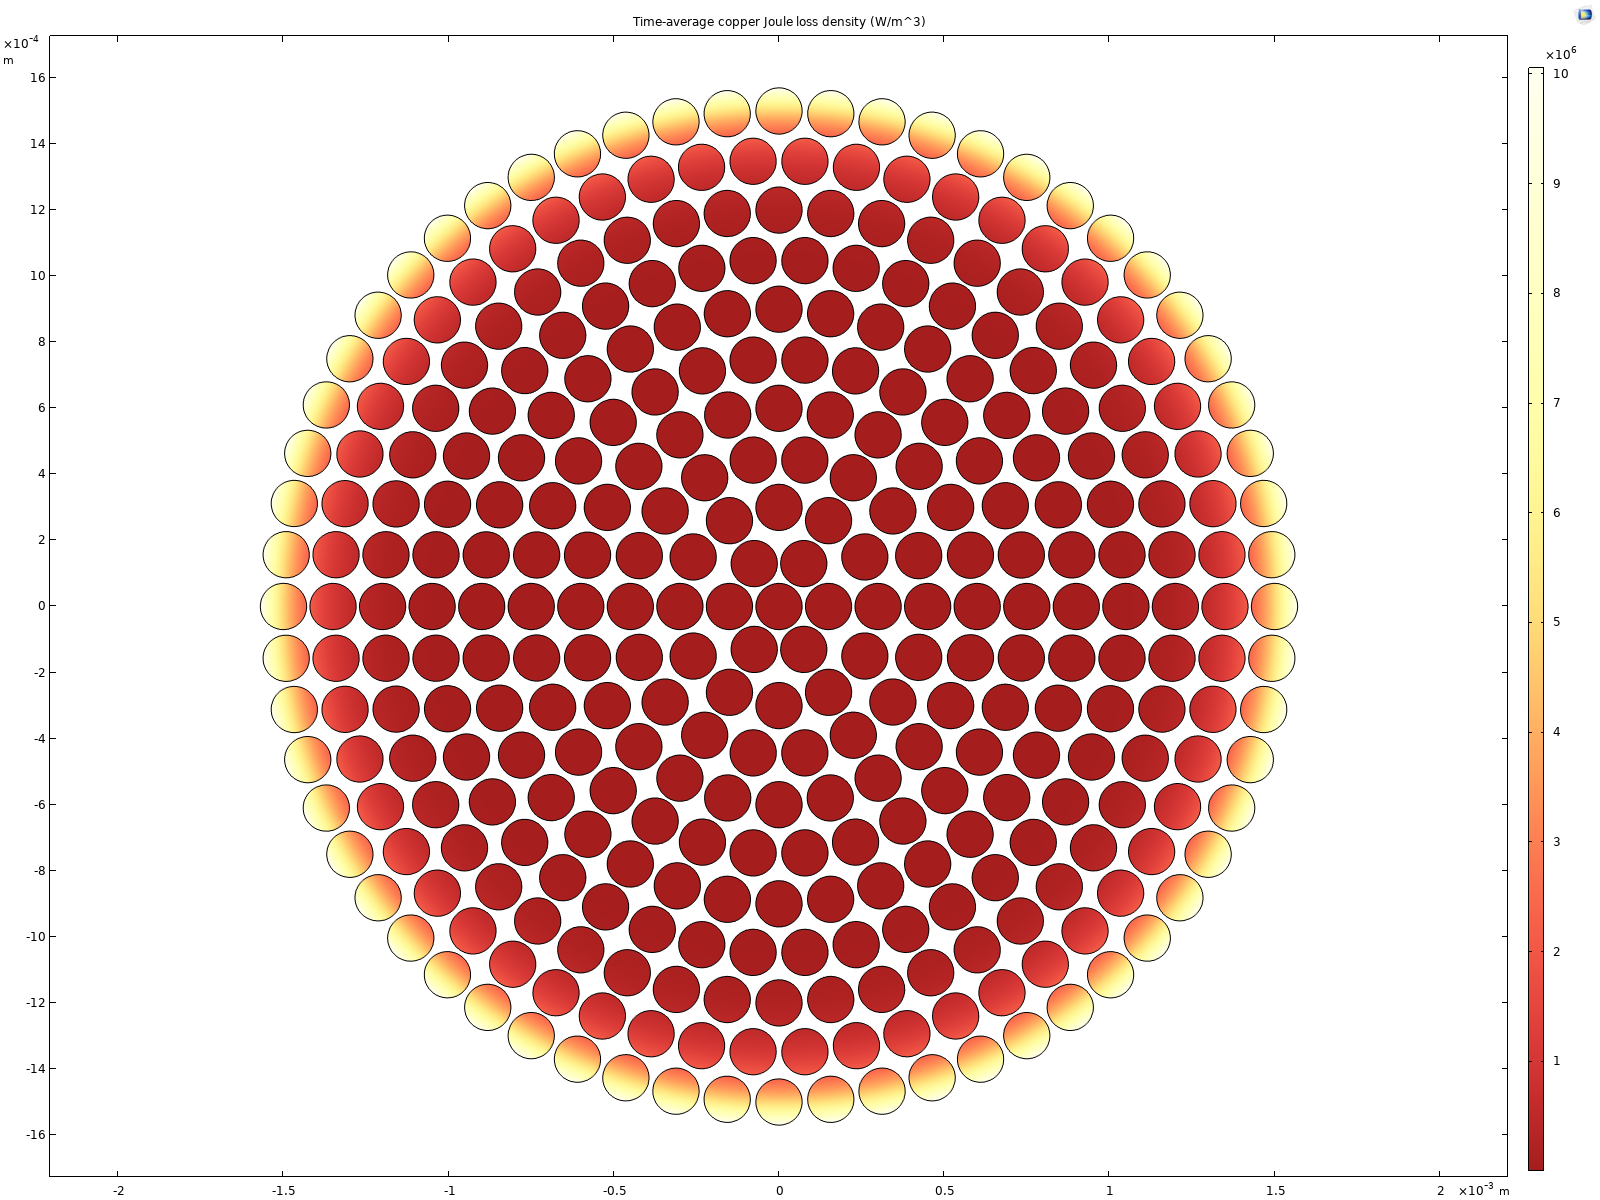
\includegraphics[width=0.92\textwidth]{figs/native_q2_loss_density.png}
\caption{圆形简单成束中的铜损密度分布（COMSOL 原生云图）。
损耗高度集中在外圈股线，与图 \ref{fig:q2-ring-loss} 的定量统计一致，
直观印证了「外圈股线是热瓶颈」的判断。}
\label{fig:q2-loss-density}
\end{figure}

\subsection{股间电流不均的机理分析}
\label{sec:q2-imbalance}

\subsubsection{逐股电流的实测结果}

赛题问题二第 4 问要求讨论「各根细丝的电流是否均匀」。
本文对全部 331 股逐一提取净电流，结果列于表 \ref{tab:q2-strand}。

\begin{table}[H]
\centering
\caption{问题二：圆形简单成束的逐股电流统计（$200\U{kHz}$，$20\U{A}$ 有效值）}
\label{tab:q2-strand}
\small
\begin{adjustbox}{max width=\textwidth}
\begin{tabular}{l c}
\toprule
\textbf{指标} & \textbf{数值} \\
\midrule
理想均分单股电流 $\bar I = 20/331$   & $60.422961\U{mA}$ \\
中心股净电流有效值                   & $\mathbf{0.540183\U{mA}}$ \\
最外圈平均股电流有效值               & $\mathbf{258.560259\U{mA}}$ \\
最外圈最小股电流有效值               & $258.494075\U{mA}$ \\
最外圈最大股电流有效值               & $258.625263\U{mA}$ \\
中心股净电流 / 股铜截面              & $0.035091\U{A/mm^2}$ \\
最外圈平均净电流 / 股铜截面          & $16.796498\U{A/mm^2}$ \\
最外圈 60 股的铜损占比               & $\mathbf{80.753370\%}$ \\
最大复电流均流偏差 $\eta_I^{\mathbb{C}}$ & $\mathbf{338.187232\%}$ \\
最大电流幅值均流偏差 $\eta_I^{|\,|}$ & $328.024810\%$ \\
\bottomrule
\end{tabular}
\end{adjustbox}
\end{table}

\begin{figure}[H]
\centering
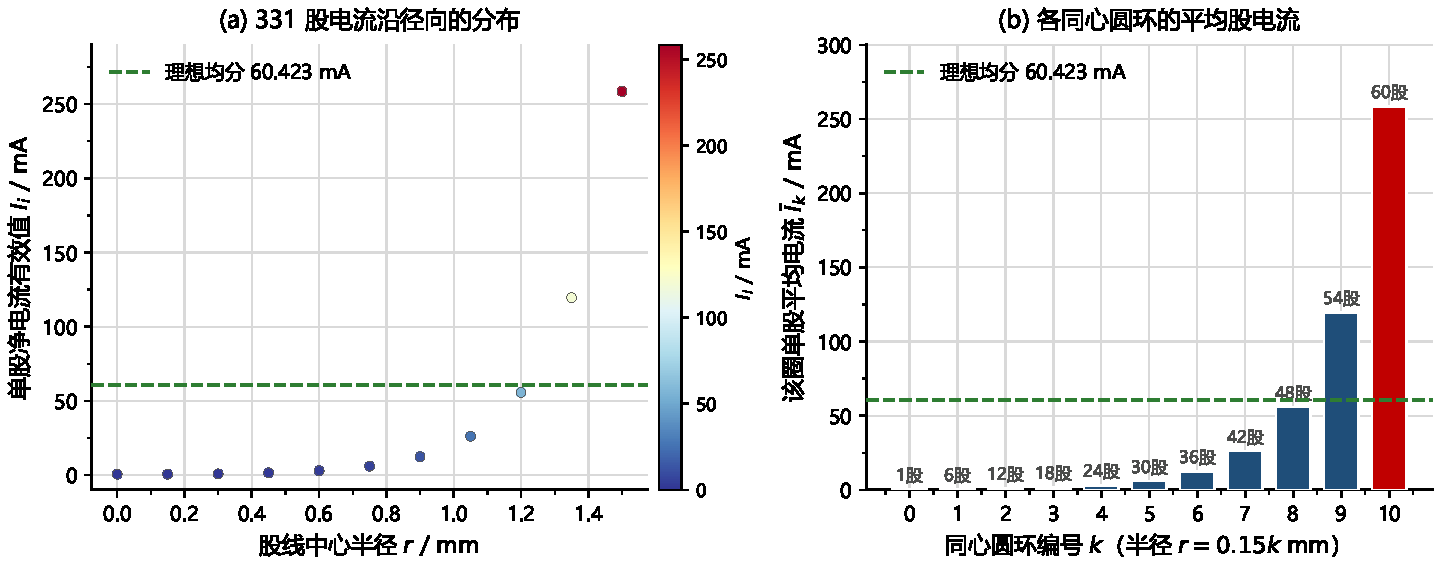
\includegraphics[width=\textwidth]{figs/q2_strand_current.pdf}
\caption{圆形简单成束的逐股电流分布。(a) 331 根股线的净电流随其中心半径的分布，
颜色表示电流大小，虚线为理想均分值 $60.423\U{mA}$；
(b) 各同心圆环的平均股电流，柱上标注该圈股数。
两者均显示电流从内向外单调急剧增大。}
\label{fig:q2-strand}
\end{figure}

\begin{figure}[H]
\centering
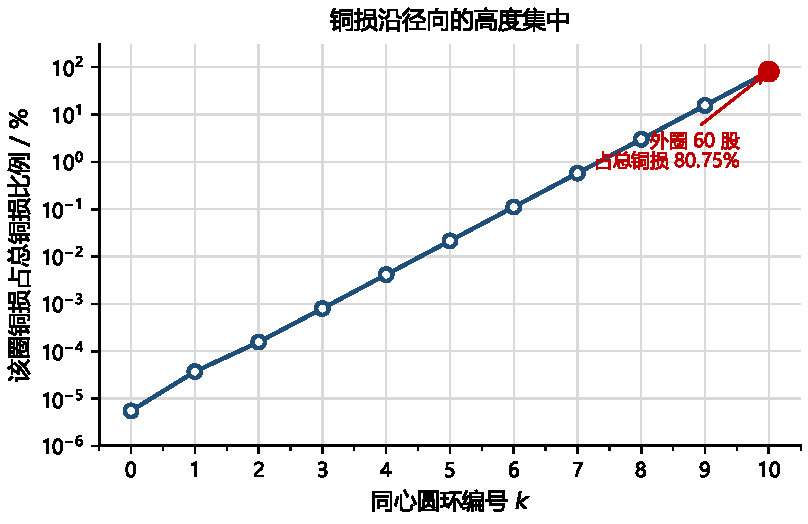
\includegraphics[width=0.58\textwidth]{figs/q2_ring_loss.pdf}
\caption{铜损沿径向的高度集中：最外圈 60 股（占总股数 $18.1\%$）
承担了 $80.75\%$ 的总铜损。纵轴为对数坐标。}
\label{fig:q2-ring-loss}
\end{figure}

\subsubsection{不均现象的量化与解读}

图 \ref{fig:q2-strand} 与表 \ref{tab:q2-strand} 给出一个\textbf{极为不平等}的电流分布：

\begin{itemize}[leftmargin=2em, itemsep=3pt]
\item 中心股仅承担 $0.540\U{mA}$，是理想值的 $0.89\%$；
\item 最外圈单股平均承担 $258.560\U{mA}$，是理想值的 \textbf{4.28 倍}；
\item 中心股与最外圈平均股之间相差 \textbf{479 倍}；
\item 最大复电流均流偏差 $\eta_I^{\mathbb{C}} = 338.19\%$，
即偏离理想值最远的那一股，其偏差达到理想电流的 $3.38$ 倍。
\end{itemize}

损耗的集中程度更为极端：\textbf{最外圈 60 股（占总股数的 $18.1\%$）
承担了 $80.75\%$ 的总铜损}，而中心区域的大量股线几乎不发热。
这意味着束内存在\textbf{严重的局部热点}——外圈股线将首先达到温度上限，
成为整根导线的热瓶颈。

\subsubsection{铜损的三分量分解}

为定量区分不同机理的贡献，本文把总铜损按每股的直流电阻与净复电流作分解：

\begin{equation}
P_{\text{总}} =
\underbrace{\sum_i |\tilde I_i|^2 R_{dc,i}}_{\text{直流基准}}
+\underbrace{\sum_i \left(|\tilde I_i|^2 - \bar I^2\right) R_{dc,i}}_{\text{股间电流不均}}
+\underbrace{\sum_i \left(P_i - |\tilde I_i|^2 R_{dc,i}\right)}_{\text{股内分布不均}} .
\label{eq:loss-decomp}
\end{equation}

\begin{table}[H]
\centering
\caption{问题二：圆形简单成束的铜损三分量分解（每米）}
\label{tab:q2-decomp}
\small
\begin{adjustbox}{max width=\textwidth}
\begin{tabular}{l c c}
\toprule
\textbf{分量} & \textbf{数值} $/\U{W/m}$ & \textbf{占总损耗} \\
\midrule
理想直流基准 $\sum_i \bar I^2 R_{dc,i}$        & $1.353499$ & $22.71\%$ \\
股间电流不均（幅值 + 相位）                    & $\mathbf{4.210570}$ & $\mathbf{70.65\%}$ \\
股内电流分布不均                               & $0.395802$ & $6.64\%$ \\
\midrule
\textbf{合计}（即 $I^2\Rac$）                  & $\mathbf{5.959871}$ & $100\%$ \\
\bottomrule
\end{tabular}
\end{adjustbox}
\end{table}

\begin{figure}[H]
\centering
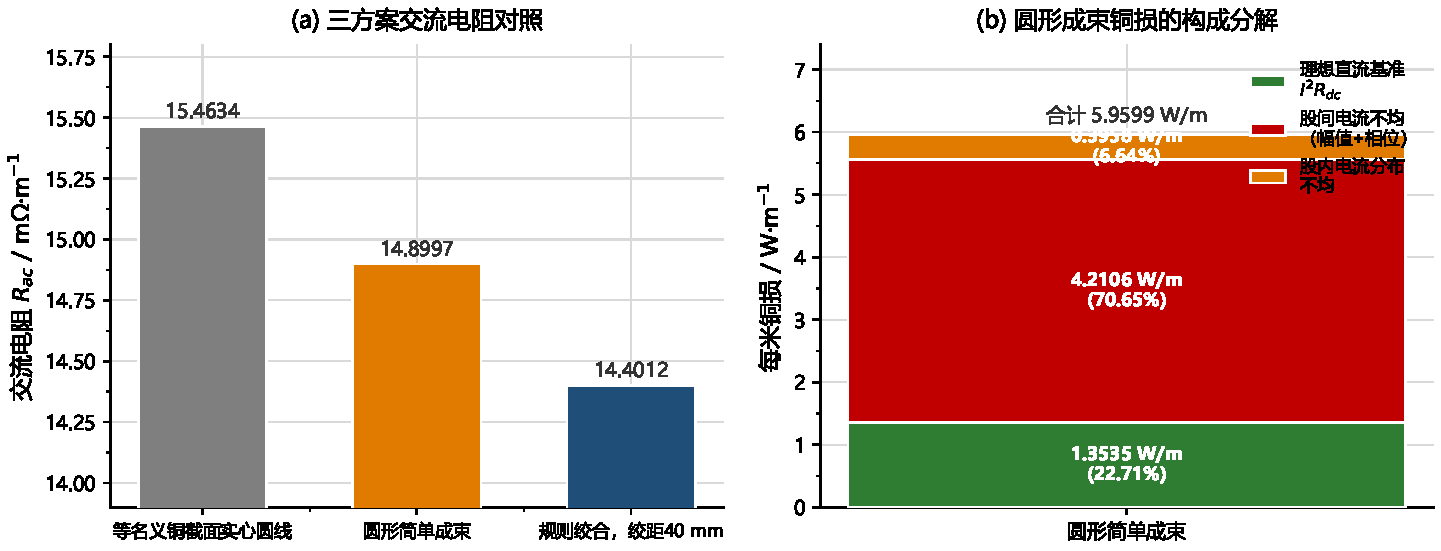
\includegraphics[width=\textwidth]{figs/q2_twist_and_decomposition.pdf}
\caption{(a) 含规则绞合的三方案交流电阻对照；
(b) 圆形成束铜损的构成分解：理想直流基准仅占 $22.71\%$，
股间电流不均贡献 $70.65\%$，是绝对主导因素。}
\label{fig:q2-decomp}
\end{figure}

这一分解给出了问题二最重要的定量结论：

\begin{tcolorbox}[colback=blue!4, colframe=blue!55!black, boxrule=0.7pt,
  arc=2pt, left=7pt, right=7pt, top=6pt, bottom=6pt]
\textbf{邻近效应的定量归因}：在圆形成束中，若各股电流完全均分、
且股内电流均匀，每米铜损应仅为 $1.3535\U{W/m}$；
实际铜损 $5.9599\U{W/m}$ 中，\textbf{有 $70.65\%$ 来自股间电流不均}，
只有 $6.64\%$ 来自股内电流分布不均。
因此，\textbf{降低损耗的主攻方向不是继续细化丝径，而是让各股电流趋于均分}——
即改善换位的彻底程度。
\end{tcolorbox}

需要谨慎说明的是，最后一项「股内电流分布不均」$0.3958\U{W/m}$
是单丝自身趋肤效应与周围股线邻近效应在\textbf{单丝内部}的叠加结果，
\textbf{不能单独称作「纯邻近效应损耗」}。

\subsection{规则绞合方案的结果}
\label{sec:q2-twist}

\subsubsection{绞合的分层电流与损耗}

\begin{table}[H]
\centering
\caption{问题二：规则绞合方案（绞距 $40\U{mm}$）的逐层统计}
\label{tab:q2-twist-strand}
\small
\begin{adjustbox}{max width=\textwidth}
\begin{tabular}{l c c}
\toprule
\textbf{指标} & \textbf{圆形简单成束} & \textbf{规则绞合（$40\U{mm}$）} \\
\midrule
理想均分单股电流                     & $60.422961\U{mA}$ & $60.422961\U{mA}$ \\
中心股电流幅值                       & $0.540183\U{mA}$  & $3.683942\U{mA}$ \\
最外层单股平均电流幅值               & $258.560259\U{mA}$ & $248.495400\U{mA}$ \\
最外层电流幅值范围                   & $258.494$--$258.625\U{mA}$ & $248.442$--$248.548\U{mA}$ \\
最外层 60 股承担的铜损               & $80.753370\%$        & $79.670429\%$ \\
截面最大实际电流密度                 & ---                  & $23.249635\U{A/mm^2}$ RMS \\
最大复电流均流偏差 $\eta_I^{\mathbb{C}}$ & $338.187232\%$   & $321.301428\%$ \\
\bottomrule
\end{tabular}
\end{adjustbox}
\end{table}

\begin{figure}[H]
\centering
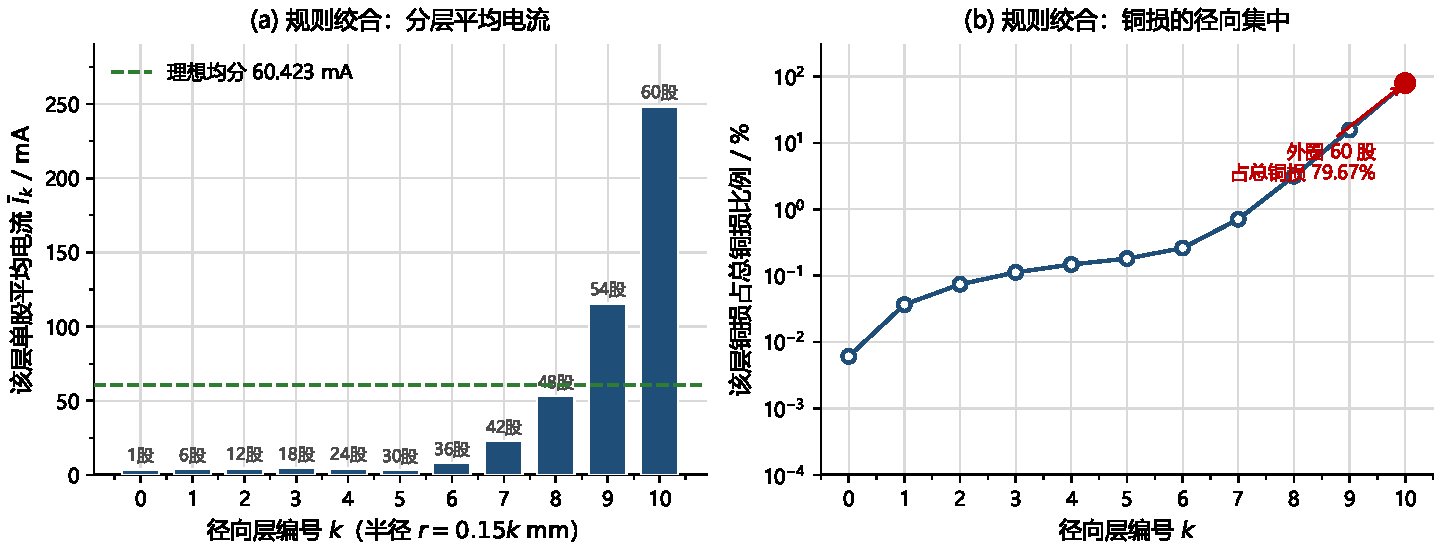
\includegraphics[width=\textwidth]{figs/q2_twist_ring.pdf}
\caption{规则绞合方案的分层电流与损耗。(a) 各径向层的平均股电流，
虚线为理想均分 $60.423\U{mA}$；
(b) 各层铜损占比（对数坐标），最外圈 60 股仍占 $79.67\%$。}
\label{fig:q2-twist-ring}
\end{figure}

\begin{figure}[H]
\centering
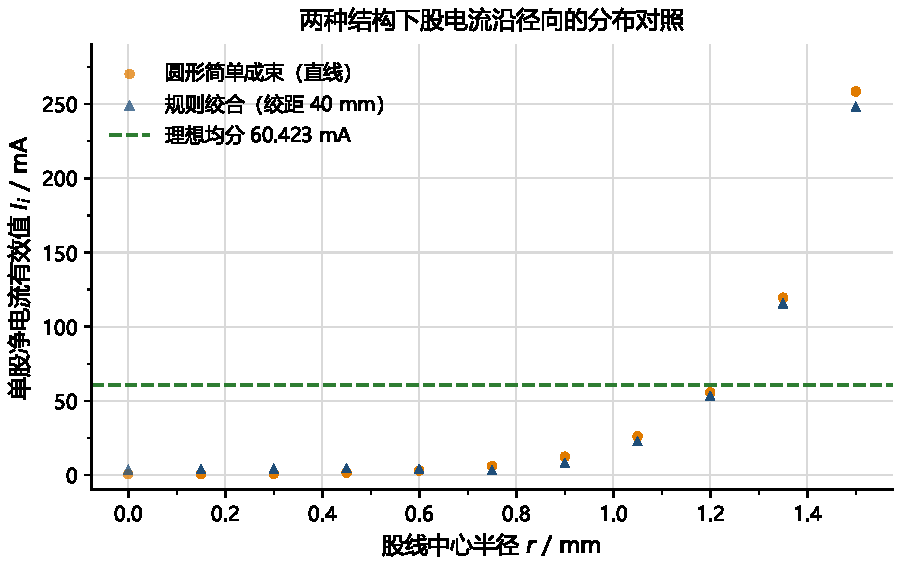
\includegraphics[width=0.72\textwidth]{figs/q2_strand_compare.pdf}
\caption{两种结构下股电流沿径向的分布对照。绞合使电流分布略微「压缩」
（外圈从 $258.56\U{mA}$ 降到 $248.50\U{mA}$，
中心股从 $0.540\U{mA}$ 升到 $3.684\U{mA}$），
但\textbf{内层清闲、外层过载的基本格局没有改变}。}
\label{fig:q2-strand-compare}
\end{figure}

\subsubsection{绞合为什么不够：几何层面的解释}

绞合确实改善了均流状况——中心股电流从 $0.540\U{mA}$ 提升到
$3.684\U{mA}$（提高 $6.82$ 倍），最大复电流均流偏差从 $338.19\%$
降到 $321.30\%$，最外圈铜损占比从 $80.75\%$ 降到 $79.67\%$。
但改善\textbf{十分有限}，因为\textbf{绞合在几何上并不改变径向层的分配}：

由式 \eqref{eq:twist-geom}，第 $k$ 层的半径 $r_k$ 是常数。
一根位于第 10 层（$r = 1.5\U{mm}$）的股线，
在整根 $1\U{m}$ 长度上虽然绕轴转了 25 圈，
但它\textbf{始终处在 $r = 1.5\U{mm}$ 这个半径上}，
始终暴露在最强的磁场中。相反，中心股始终处于 $r = 0$ 的弱场区。
绞合只让股线在\textbf{同一层内}交换方位角，
而由于本文模型是轴对称的（10 个完整圆环），
同层内的方位角交换\textbf{对电磁环境几乎没有影响}。

\begin{tcolorbox}[colback=red!4, colframe=red!60!black, boxrule=0.7pt,
  arc=2pt, left=7pt, right=7pt, top=6pt, bottom=6pt]
\textbf{核心结论（直接引出问题三）}：绞合之所以无法把 $\Rac/\Rdc$ 压到接近 1，
不是因为绞合「没起作用」，而是因为它的\textbf{换位是不彻底的}——
股线的径向轨迹 $r(z) \equiv r_k$ 恒为常数，
内外层之间没有任何交换。
要把 $\Rac/\Rdc$ 压向理想值，必须让每股的轨迹满足
$r(z)$ 在结构周期内\textbf{真正遍历所有径向层}，
即采用三维轨迹 $(r(z), \theta(z), z)$ 的\textbf{三维拓扑编织}。
这正是问题三的任务。
\end{tcolorbox}

\begin{figure}[H]
\centering
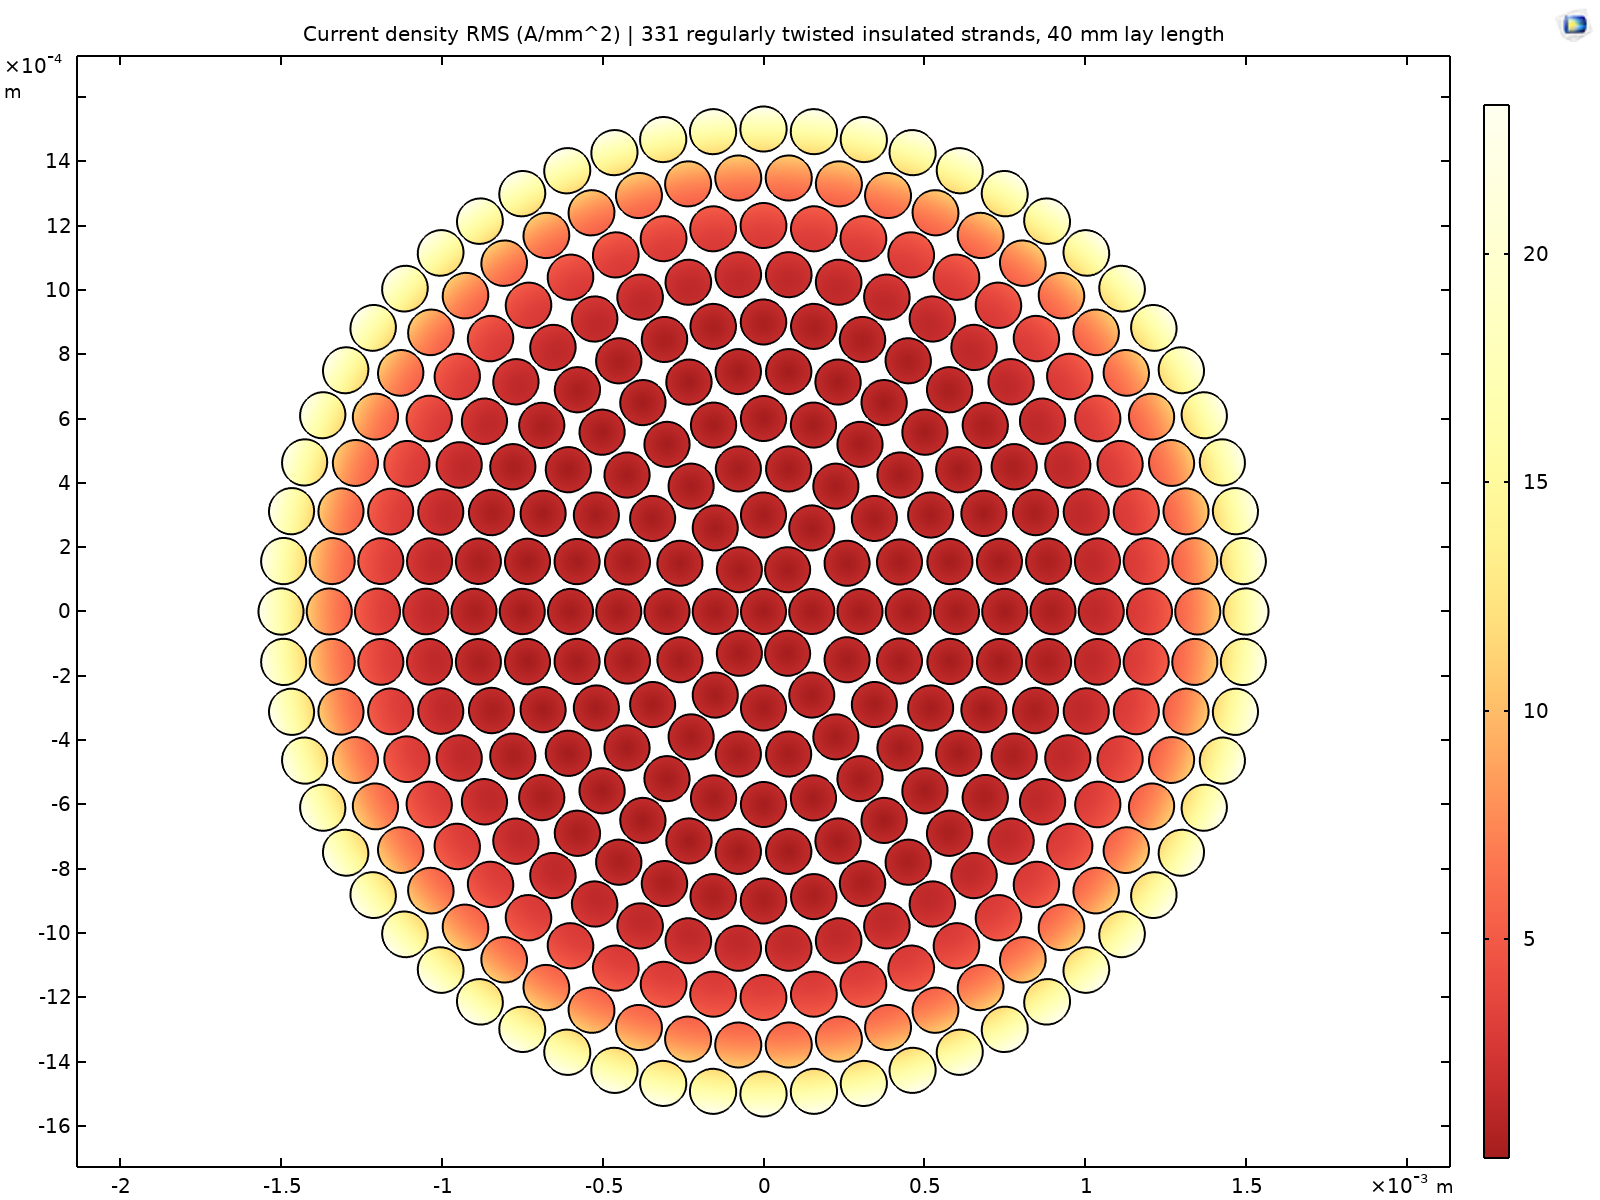
\includegraphics[width=0.92\textwidth]{figs/native_q2_twist_current_density.png}
\caption{规则绞合方案中各股内部的局部电流密度有效值分布（COMSOL 原生云图）。
绞合引入了周向电流分量，单股内部电流分布与简单成束有所不同。}
\label{fig:q2-twist-local-j}
\end{figure}

\begin{figure}[H]
\centering
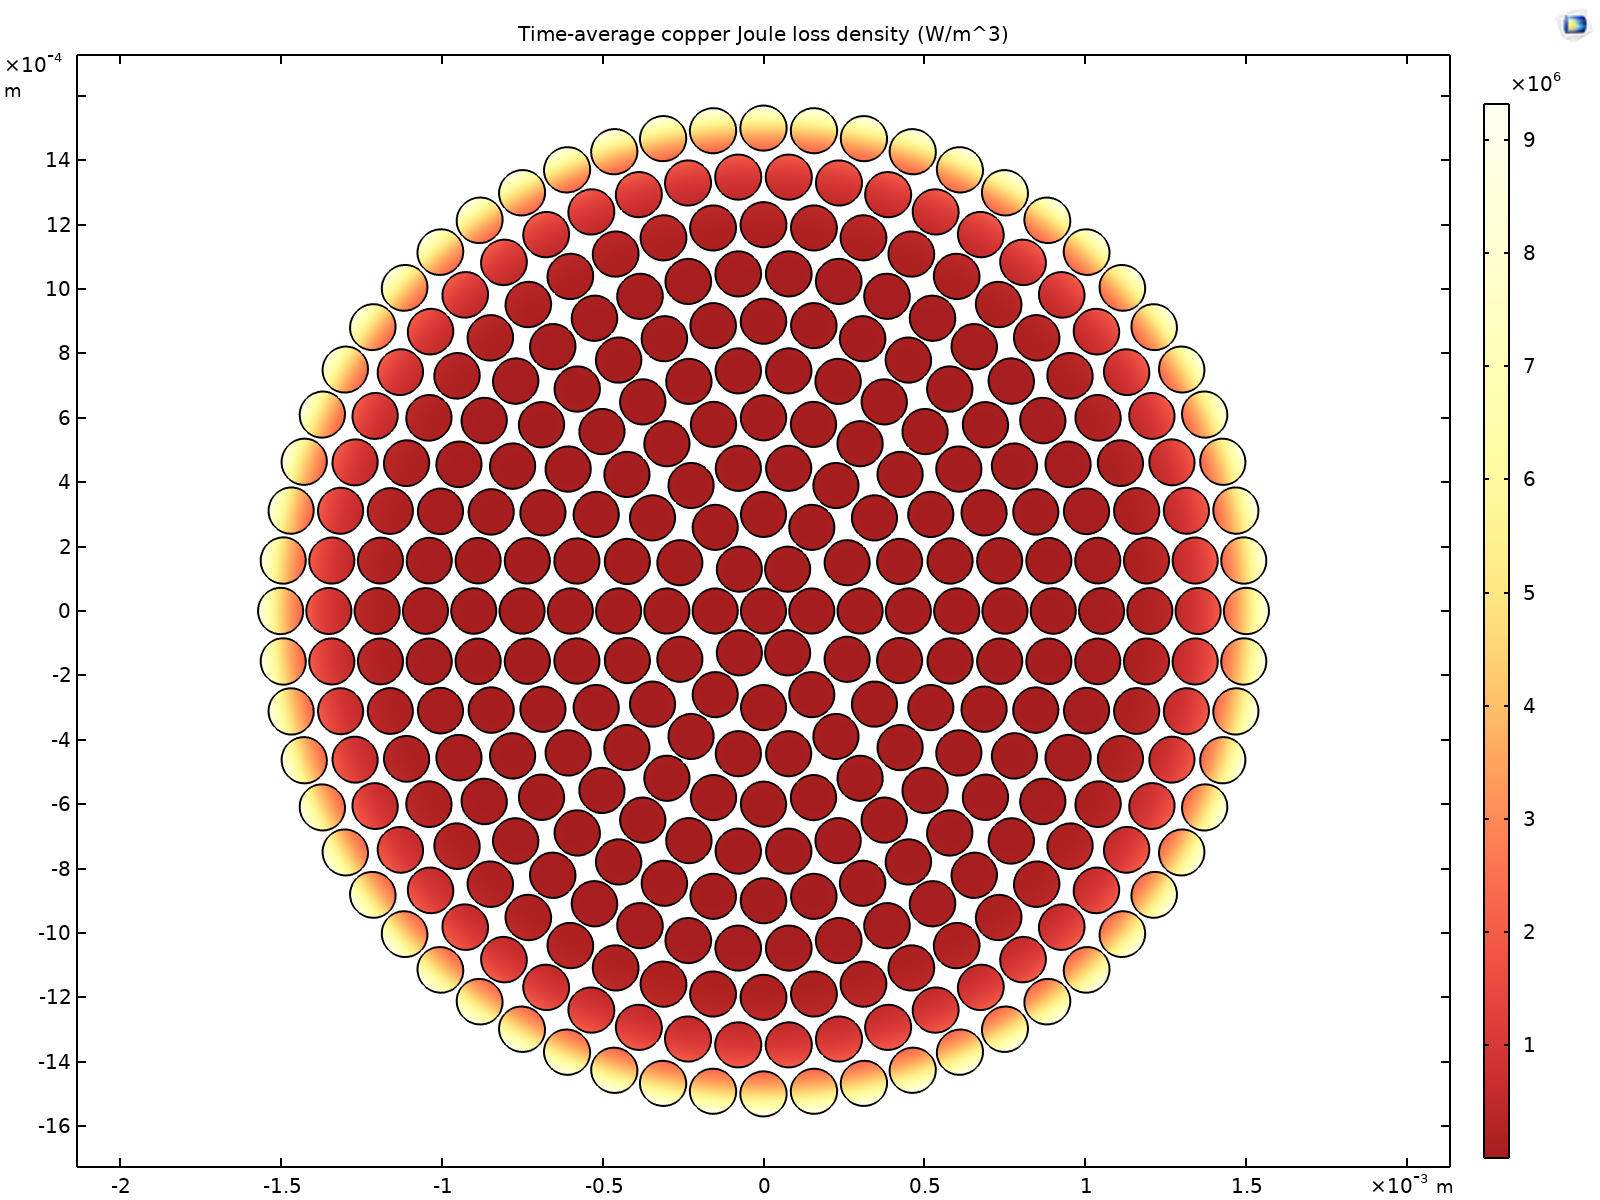
\includegraphics[width=0.92\textwidth]{figs/native_q2_twist_loss_density.png}
\caption{规则绞合方案的铜损密度分布（COMSOL 原生云图）。
与图 \ref{fig:q2-loss-density} 对比可见，绞合虽略微缓解了外圈集中，
但未改变「内层清闲、外层过载」的基本格局。}
\label{fig:q2-twist-loss}
\end{figure}

\subsection{数值校验}
\label{sec:q2-verify}

赛题要求「所有关键结论必须可由提交的仿真工程文件或原始导出数据复现」。
本文对两种方案均做了系统校验，结果列于表 \ref{tab:q2-verify}。

\begin{table}[H]
\centering
\caption{问题二：数值校验汇总}
\label{tab:q2-verify}
\small
\begin{adjustbox}{max width=\textwidth}
\begin{tabular}{l l l}
\toprule
\textbf{校验项} & \textbf{圆形简单成束} & \textbf{规则绞合} \\
\midrule
网格：后两档 $\Rac$ 相对变化 & $0.00028070\%$ & $0.00028814\%$ \\
主模型自由度                 & 176142 & 660587 \\
外边界半径 $20\to40\U{mm}$ 对 $\Rac$ 影响 & $1.18\times10^{-7}\%$ & $0.021255\%$ \\
零绞度极限（与原直线模型差） & --- & $6.73\times10^{-5}\%$ \\
低频极限（$10\U{Hz}$）$\Rac/\Rdc$ & $1.000006999$ & $1.000006553$ \\
$10\U{Hz}$ 各股电流幅值最大相对偏差 & $0.00006065\%$ & --- \\
$10\U{Hz}$ 复电流最大相对偏差 & $0.093655\%$ & --- \\
$331$ 股复电流之和           & $20 - j3.30\times10^{-12}\U{A}$ & $20 + j1.50\times10^{-12}\U{A}$ \\
铜损法与终端电压法提取电阻之差 & $1.20\times10^{-11}$ & --- \\
功率平衡相对残差             & $1.20\times10^{-11}$ & $1.73\times10^{-11}$ \\
逐股损耗之和 vs 总积分       & 一致 & 一致 \\
文件回读                     & --- & 通过 \\
\bottomrule
\end{tabular}
\end{adjustbox}
\end{table}

各项校验的物理含义：

\begin{enumerate}[label=(\arabic*), leftmargin=2.2em, itemsep=3pt]
\item \textbf{网格收敛}：两种方案后两档网格的 $\Rac$ 相对变化均低于
$0.0003\%$，说明离散误差已可忽略。
\item \textbf{低频极限}：$10\U{Hz}$ 时趋肤与邻近效应均可忽略，
$\Rac/\Rdc$ 应趋于 1。实测圆形成束 $1.000006999$、
绞合 $1.000006553$（后者符合螺旋线长公式给出的修正），
\textbf{证实模型在高频与低频两个极限下都是正确的}，
且低频下的电流分布确实趋于完全均分（幅值偏差仅 $6\times10^{-5}\%$）。
\item \textbf{零绞度极限}：把绞率置零后，绞合模型退化为直线模型，
与圆形成束的 $\Rac$ 相差 $6.73\times10^{-5}\%$，
说明螺旋坐标降维方法在极限情况下\textbf{不会引入额外误差}。
\item \textbf{边界截断}：外边界半径由 $20\U{mm}$ 增至 $40\U{mm}$，
圆形成束的 $\Rac$ 变化仅 $1.18\times10^{-7}\%$，
说明 $20\U{mm}$ 的空气域已足够大。绞合方案为 $0.0213\%$，
略大但仍可接受（因绞合存在周向电流，外部场衰减稍慢）。
\item \textbf{电流守恒与功率平衡}：331 股复电流之和等于 $20\U{A}$，
铜损法与终端电压法提取的电阻一致，功率平衡残差在 $10^{-11}$ 量级，
\textbf{说明后处理提取的正确性}。
\end{enumerate}

需要诚实说明的是，以上校验支持\textbf{当前离散模型}的数值稳定性与内部一致性，
\textbf{不代表}端部效应、外部回流、热学等未建模因素的误差上限。

\subsection{问题二小结}

问题二的核心结论可概括为三点：

\begin{enumerate}[label=(\arabic*), leftmargin=2.2em, itemsep=3pt]
\item \textbf{设计依据清晰可追溯}：由 $\beta = d/\delta = 0.9474 < 1$ 定丝径
$d = 0.14\U{mm}$，由 $J_{dc}\le 4\U{A/mm^2}$ 定最小铜截面 $5\U{mm^2}$
（$\ge 325$ 股），由六重对称与可制造性（最小间隙 $10\U{\mu m}$）定 $N = 331$。
\item \textbf{Litz 化有收益但远未达理想}：圆形束 $\Rac/\Rdc = 4.4033$
vs 等铜截面实心线 $4.5699$，仅改善 $3.65\%$；
规则绞合进一步到 $4.1931$，累计改善 $6.87\%$，
但相对理想值 $1.00$ 仍差 $3.2$ 倍。
\item \textbf{不均的机理已被定量定位}：股间电流不均贡献了 $70.65\%$ 的铜损，
是绝对主导因素；最外圈 $18.1\%$ 的股线承担 $80.75\%$ 的损耗，
存在严重局部热点风险。绞合由于径向层固定而无法解决这一问题。
\end{enumerate}

% =====================================================================
%  五、问题三（框架，待补）
% =====================================================================
\section{问题三：编织方案的仿真调优}
\label{sec:q3}

\begin{todobox}[本节状态说明]
问题三为开放性优化题（30 分），要求以仿真为实验手段系统搜索编织参数空间。
其完整的参数化建模、仿真迭代、方案对比与敏感性分析\textbf{尚在执行中}。
本节先行确定评价指标体系与技术路线，正文数据待补充。
\textbf{本节不含任何仿真结果，请勿引用为已完成结论。}
\end{todobox}

\subsection{评价目标的定义}

在等总铜截面、等频率、等激励的约束下，以 $\Rac/\Rdc$ 最小化为\textbf{核心目标}，
并补充以下辅助指标：

\begin{table}[H]
\centering
\caption{问题三拟采用的评价指标体系}
\label{tab:q3-metrics}
\small
\begin{adjustbox}{max width=\textwidth}
\begin{tabular}{c l l l}
\toprule
\textbf{类型} & \textbf{指标} & \textbf{定义} & \textbf{作用} \\
\midrule
核心 & $\Rac/\Rdc$ & 见 \S\ref{sec:q1-result} & 损耗水平的综合度量 \\
辅助 & 均流偏差 $\eta_I$ & 式 \eqref{eq:eta} & 换位公平性的直接度量 \\
辅助 & 每米损耗 $P$ & $P = I^2\Rac$ & 工程发热量 \\
辅助 & 损耗集中度 & 最外圈铜损占比 & 热点风险评估 \\
辅助 & 换位充分性 $D_{\mathrm{shell}}$ & 各股径向壳层停留分布 & 问题四判据的接口 \\
 & & 与面积加权均匀分布的偏差 & \\
\bottomrule
\end{tabular}
\end{adjustbox}
\end{table}

其中换位充分性 $D_{\mathrm{shell}}$ 的形式化定义将直接为问题四的
「完美换位」判据提供接口，其定义式将在 \S\ref{sec:q4} 中给出。

\subsection{设计变量}

拟考察的设计变量包括：

\begin{itemize}[leftmargin=2em, itemsep=2pt]
\item 股数 $N$ 与丝径 $d$（在等总铜截面约束下二者联动，$N d^2 = \text{const}$）；
\item 编织角（股线螺旋方向与缆轴线的夹角），决定径向行程与结构周期；
\item 换位周期（每股完成一次「外层$\to$内层$\to$外层」循环所需的轴向长度）；
\item 单层 / 多层结构，以及子束的分层方式；
\item 径向壳层的划分方式与每股在各壳层的停留时间分配。
\end{itemize}

\subsection{调优闭环}

拟建立的迭代流程为：\textbf{设计参数 $\to$ 程序化三维几何建模 $\to$
电磁仿真（涡流场 / 坐标降维）$\to$ 指标评估（$\Rac/\Rdc$、均流）$\to$ 修改参数}，
循环至指标收敛。方案间比较\textbf{严格控制变量}（同总铜截面、同频率、同激励），
每个进入论文的结论都必须有对应仿真数据支撑。

\subsection{待补内容清单}

\begin{itemize}[leftmargin=2em, itemsep=2pt]
\item \todo{至少 3 种本质不同的换位/编织方案的三维几何建模与参数化脚本}
\item \todo{各方案在 $200\U{kHz}$、$20\U{A}$、等铜截面下的 COMSOL 仿真结果}
\item \todo{方案间 $\Rac/\Rdc$、$\eta_I$、损耗集中度的同约束对比表与对照图}
\item \todo{最优方案的参数报告与论证}
\item \todo{关键参数（编织角、换位周期）对指标的敏感性分析}
\item \todo{完整的「设计—仿真—评估」迭代数据表与日志}
\end{itemize}

% =====================================================================
%  六、问题四（框架，待补）
% =====================================================================
\section{问题四：追寻「完美编织」与成果展示网站}
\label{sec:q4}

\begin{todobox}[本节状态说明]
问题四为全开放探索题（35 分），要求提出「完美换位」的数学判据、
设计逼近该判据的编织拓扑、进行仿真验证并搭建展示网站。
本节\textbf{尚在执行中}，以下仅列出已确定的框架与待补内容，
\textbf{不含任何仿真结果或网站链接。}
\end{todobox}

\subsection{「完美换位」判据的拟定方向}

赛题提示可从「每根丝在各径向壳层上的停留分布、方位角覆盖」等角度形式化表述。
本文拟沿以下方向构造判据：

设把束截面按半径划分为 $M$ 个径向壳层 $\{S_1,\dots,S_M\}$，
壳层 $S_m$ 的面积为 $A_m$。第 $i$ 股在结构周期 $L_c$ 内于壳层 $S_m$ 中的停留弧长为
$\ell_{i,m}$，定义其\textbf{壳层停留占比}

\begin{equation}
p_{i,m} = \frac{\ell_{i,m}}{\sum_{m'=1}^{M}\ell_{i,m'}} .
\label{eq:shell-occupancy}
\end{equation}

若「电磁履历一致」等价于「各股在各壳层的停留时间与壳层面积成正比」，
则完美换位要求

\begin{equation}
p_{i,m} = \frac{A_m}{\sum_{m'=1}^{M} A_{m'}}
\qquad \forall\, i,\, m ,
\label{eq:perfect}
\end{equation}

据此定义\textbf{换位充分性偏差}

\begin{equation}
D_{\mathrm{shell}} = \max_{i} \sum_{m=1}^{M}
\left| p_{i,m} - \frac{A_m}{A_{\mathrm{tot}}} \right| ,
\label{eq:Dshell}
\end{equation}

理想完美编织对应 $D_{\mathrm{shell}} = 0$。
式 \eqref{eq:perfect} 的物理依据是：邻近效应损耗近似与股线所处位置的
磁场强度平方成正比，而磁场强度与距轴距离相关，
因此「按壳层面积加权均匀停留」可使各股的\textbf{平均磁场暴露水平}趋于一致，
从而均分电流与损耗。该判据的可计算性与合理性论证、
以及是否需引入方位角覆盖的补充条件，将在完整版中给出。

\subsection{待补内容清单}

\begin{itemize}[leftmargin=2em, itemsep=2pt]
\item \todo{「完美换位」判据的完整数学定义、可计算性证明与合理性论证}
\item \todo{逼近该判据的三维编织拓扑设计（交叉序列 / braid word、逐站截面状态、股线轨迹方程）}
\item \todo{该拓扑的电磁仿真验证，与问题三最优方案在同约束下的对比与差距报告}
\item \todo{可制造性讨论（运动/事件序列、层间交换、「拓扑 $\to$ 事件 $\to$ 轨迹」分层）}
\item \todo{成果展示网站：公开 URL、源码包、物理可视化、三维交互展示}
\end{itemize}

% =====================================================================
%  七、结果与讨论
% =====================================================================
\section{结果与讨论}

\subsection{已获得结果汇总}

本文已完成问题一、问题二的完整建模、仿真与验证，核心数据汇总于表
\ref{tab:all-results}。所有数值均来自本机 COMSOL Multiphysics 6.2 的真实有限元求解，
可由随文提交的 \texttt{.mph} 工程文件与原始导出 CSV 完整复现。

\begin{table}[H]
\centering
\caption{问题一、问题二核心结果汇总（$f = 200\U{kHz}$，$I = 20\U{A}$ 有效值，$L = 1\U{m}$）}
\label{tab:all-results}
\small
\begin{adjustbox}{max width=\textwidth}
\begin{tabular}{l c c c c c}
\toprule
\textbf{结构} & \textbf{铜截面} & $\Rdc$ & $\Rac$ & $\Rac/\Rdc$ & \textbf{每米铜损} \\
 & $/\U{mm^2}$ & $/\Umohm$ & $/\Umohm$ & & $/\U{W}$ \\
\midrule
实心线 $\varnothing 2\U{mm}$（问题一） & 3.141593 & 5.488101 & 20.016203 & 3.647200 & 8.006481 \\
\midrule
\multicolumn{6}{l}{\textit{以下三行为等铜截面对照组（$A = 5.095349\U{mm^2}$）}} \\
等铜截面实心线 $\varnothing 2.5471\U{mm}$ & 5.095349 & 3.383748 & 15.463402 & 4.569903 & 6.185361 \\
六边形简单成束（331 股）                     & 5.095349 & 3.383748 & 15.762611 & 4.658328 & 6.305045 \\
圆形简单成束（331 股，本文基线）             & 5.095349 & 3.383748 & 14.899678 & 4.403305 & 5.959871 \\
\midrule
规则绞合（331 股，绞距 $40\U{mm}$）       & 5.095349$^{*}$ & 3.434493 & 14.401182 & 4.193102 & 5.760473 \\
\bottomrule
\multicolumn{6}{l}{\footnotesize $^{*}$ 绞合方案的名义铜截面与对照组相同，
但每轴向米铜体积因螺旋而增加 $1.507\%$（$5.172137\U{mm^3/mm}$）。}
\end{tabular}
\end{adjustbox}
\end{table}

\subsection{关于换位效果的讨论}

本文通过问题一、问题二的实测数据，建立了如下递进的证据链：

\begin{enumerate}[label=\textbf{证据\arabic*}, leftmargin=4.4em, itemsep=4pt]
\item \textbf{趋肤效应确实存在且量级严重}。$2\U{mm}$ 实心铜线在
$200\U{kHz}$ 下 $\Rac/\Rdc = 3.6472$，表面与轴心电流密度相差 113 倍，
中心铜材几乎完全闲置（\S\ref{sec:q1-result}）。
\item \textbf{细径化是必要但不充分的}。$0.14\U{mm}$ 单丝的孤立
$\Rac/\Rdc$ 仅 $1.00105$，即单丝内部趋肤效应几乎消除（\S\ref{sec:q2-compare}）；
但 331 股成束后的实测 $\Rac/\Rdc = 4.4033$，
\textbf{说明损耗的来源已经发生了转移}——从「丝内」转移到了「丝间」。
\item \textbf{丝间损耗的绝对主导项是股间电流不均}。铜损分解表明，
理想直流基准仅 $1.3535\U{W/m}$，股间电流不均贡献 $4.2106\U{W/m}$
（占 $70.65\%$），股内分布不均仅 $0.3958\U{W/m}$（占 $6.64\%$）
（\S\ref{sec:q2-imbalance}）。\textbf{这一定量归因是本文最具指导意义的发现}：
它说明后续优化的重心应放在\textbf{改善换位、均分电流}，
而非继续细化丝径或增加股数。
\item \textbf{绞合提供的换位不彻底}。绞距 $40\U{mm}$ 的规则绞合把
$\Rac/\Rdc$ 从 $4.4033$ 改善到 $4.1931$（降低 $3.35\%$），
但中心股与外圈平均电流之比仍为 $1:67.5$，
外圈 60 股仍占 $79.67\%$ 的铜损（\S\ref{sec:q2-twist}）。
几何分析表明根源在于 $r(z) \equiv r_k$ 恒为常数，
股线\textbf{从未跨层}。
\item \textbf{因此需要真正的三维换位}。要把 $\Rac/\Rdc$ 压向理想值，
必须让每股轨迹在结构周期内真正遍历所有径向层，
即 $r(z)$ 非常数——这正是三维拓扑编织的定义，
也是问题三、四的技术路线依据。
\end{enumerate}

\subsection{结果的可信度与局限}

\textbf{可信度支撑}：

\begin{itemize}[leftmargin=2em, itemsep=2pt]
\item 问题一的有限元结果与 Bessel 精确解在全部径向采样点上
最大相对误差 $1.28\times10^{-6}\%$，复相量分量亦吻合；
\item 网格收敛性经五档独立求解确认，最终档的网格变化影响 $<2\times10^{-5}\%$；
\item 问题二两个方案均通过低频极限、电流守恒、功率平衡、
外边界截断与文件回读五项校验，残差均在 $10^{-11}$ 量级；
\item 绞合方案通过零绞度极限校验（$6.73\times10^{-5}\%$），
确认坐标降维方法不引入额外误差。
\end{itemize}

\textbf{已识别的局限}（本文所有结论均在此范围内成立）：

\begin{enumerate}[label=(\arabic*), leftmargin=2.2em, itemsep=3pt]
\item \textbf{端部效应未建模}。模型描述的是均匀长直导线的一段，
端部接线端子、端部场畸变与实际回路的外部回流导体均未纳入，
\textbf{电感与电压虚部的绝对值依赖所取外部场参考，
不代表实际回路的测量值}。
\item \textbf{热电解耦}。未计算温升，$J_{dc}\le 4\U{A/mm^2}$
仅作为截面选择的\textbf{直流意义}约束，不能替代实际高频热仿真。
实际外圈股线的局部电流密度远高于 $J_{dc}$，
真实温升将高于按平均电流密度的估计。
\item \textbf{漆膜未建模}。$10\U{\mu m}$ 的几何间隙等效表示绝缘，
未建立漆膜的介电与热学模型。
\item \textbf{螺旋坐标降维的适用范围}。该方法适用于同旋向、同绞距、
固定半径的结构；径向换位、不同绞距或多级子束需重新核查其适用性。
\item \textbf{六边形对照数据为沿用值}。问题二中六边形简单成束与
等铜截面实心线的结果沿用上一版已验证的求解结果
（原始数据与校验值随包附上，见 \texttt{reference\_hexagonal/}），
\textbf{本次未重新求解}；圆形与绞合方案为本次实际求解。
\item \textbf{问题三、四尚无仿真结果}。本文不包含任何编织方案的调优数据，
相关章节仅提供框架。
\end{enumerate}

% =====================================================================
%  八、结论
% =====================================================================
\section{结论}

本文以真实有限元仿真为唯一证据来源，完成了赛题问题一与问题二的
「建模—仿真—验证」全流程，主要工作与结论如下。

\textbf{（一）问题一：建立了可信的高频电磁仿真基准。}
推导得 $200\U{kHz}$ 下铜的趋肤深度 $\delta = 147.772\U{\mu m}$。
对 $\varnothing 2\U{mm}$、$1\U{m}$ 实心圆铜导线建模求解，得
$\Rac = 20.0162\Uohm$、$\Rac/\Rdc = 3.6472$、$P = 8.0065\U{W/m}$。
径向网格由 8 加密至 128，$\Rac$ 单调收敛，最后两档相对变化
$1.92\times10^{-5}\%$，与 Bessel 精确解的相对误差 $1.28\times10^{-6}\%$，
径向复电流密度最大误差为表面幅值的 $0.0394\%$。
按 $1/e$ 判据定义的电流集中层厚度为 $160.983\U{\mu m}$，
与圆柱精确解相差 $0.011\U{\mu m}$，比平面波 $\delta$ 大 $8.94\%$，
该差异可由 $a/\delta\approx6.77$ 的曲率效应完全解释。
$50\U{kHz}$--$1\U{MHz}$ 七频点扫描与解析解最大误差 $4.30\times10^{-5}\%$。

\textbf{（二）问题二：完成了 Litz 线的定量设计与实测评估。}
以 $\beta = d/\delta = 0.9474 < 1$ 定丝径 $d = 0.14\U{mm}$，
以 $J_{dc}\le4\U{A/mm^2}$ 定最小铜截面 $5\U{mm^2}$（$\ge325$ 股），
取十层同心圆环得 $N = 331$、总铜截面 $5.0953\U{mm^2}$、
最小丝间间隙 $10\U{\mu m}$。
实测圆形简单成束 $\Rac = 14.8997\Uohm$、$\Rac/\Rdc = 4.4033$，
相对等铜截面实心线改善 $3.65\%$；
规则绞合（绞距 $40\U{mm}$）$\Rac = 14.4012\Uohm$、
$\Rac/\Rdc = 4.1931$，相对实心线累计改善 $6.87\%$。

\textbf{（三）给出了邻近效应的定量归因。}
铜损分解表明，圆形成束的总损耗 $5.9599\U{W/m}$ 中，
理想直流基准仅 $1.3535\U{W/m}$（$22.71\%$），
\textbf{股间电流不均贡献 $4.2106\U{W/m}$（$70.65\%$）}，
股内电流分布不均贡献 $0.3958\U{W/m}$（$6.64\%$）。
逐股数据显示中心股仅 $0.540\U{mA}$、最外圈平均 $258.560\U{mA}$
（理想值 $60.423\U{mA}$），最大复电流均流偏差 $338.19\%$，
最外圈 $18.1\%$ 的股线承担 $80.75\%$ 的铜损。

\textbf{（四）从几何上阐明了绞合为何不彻底，并据此确定后续路线。}
绞合中 $r(z)\equiv r_k$ 恒为常数，股线只做等半径螺旋运动，
径向层永不交换，故绞合虽降低损耗 $3.35\%$，
但内层清闲、外层过载的基本格局未变（外圈仍占铜损 $79.67\%$）。
由此得出核心判断：\textbf{把 $\Rac/\Rdc$ 压向 1 的决定性手段是结构性换位，
必须让股线轨迹 $r(z)$ 在结构周期内真正遍历所有径向层}，
即三维拓扑编织。本文实测得到的两条基线（成束 $4.4033$、绞合 $4.1931$）
为问题三的方案搜索提供了可比较的起点。

\textbf{（五）问题三、问题四的执行状态。}
本文已为问题三确定了以 $\Rac/\Rdc$ 为核心、
辅以 $\eta_I$、损耗集中度与换位充分性 $D_{\mathrm{shell}}$ 的指标体系，
以及参数化建模与调优闭环的技术路线；为问题四拟定了
基于壳层停留占比的「完美换位」判据形式（式 \eqref{eq:perfect}--\eqref{eq:Dshell}）。
\textbf{两题的仿真数据、方案对比与展示网站尚在执行中，本文不含相关结论。}

% =====================================================================
%  参考文献
% =====================================================================
\newpage
\begin{thebibliography}{99}
\addcontentsline{toc}{section}{参考文献}

\bibitem{comsol-mfh}
COMSOL AB. \textit{AC/DC Module User's Guide — Magnetic Field Formulation,
Version 6.2}. Stockholm: COMSOL AB, 2023.
\url{https://doc.comsol.com/6.2/doc/com.comsol.help.acdc/}

\bibitem{comsol-gauge}
COMSOL AB. \textit{How Do I Use Gauge Fixing in COMSOL Multiphysics?}
COMSOL Blog, 2023.
\url{https://www.comsol.com/blogs/how-do-i-use-gauge-fixing-in-comsol-multiphysics/}

\bibitem{bessel}
Sullivan C R. Computationally efficient winding loss calculation with
multiple windings, arbitrary waveforms, and two-dimensional field geometry.
\textit{IEEE Transactions on Power Electronics}, 2001, 16(1): 142--150.

\bibitem{litz}
Sullivan C R. \textit{Cost-constrained selection of strand diameter and number
in a litz-wire transformer winding}. IEEE Transactions on Power Electronics,
1999, 14(2): 281--288.

\bibitem{fem-cable}
Finite Element Modeling of Power Cables using Coordinate Transformations.
arXiv:2307.00814, 2023.
\url{https://arxiv.org/abs/2307.00814}

\bibitem{skin-classic}
Lammeraner J, \v{S}tafl M. \textit{Eddy Currents}. London: Iliffe Books, 1966.

\bibitem{ctma}
CTMA / K-TLitz 三维拓扑编织研究项目. 命题背景支持资料, 2026.

\bibitem{comsol-three-comp}
COMSOL AB. \textit{Magnetic Field Formulation: Three-Component Formulation},
Version 6.2. \url{https://doc.comsol.com/6.2/doc/com.comsol.help.acdc/}

\end{thebibliography}

% =====================================================================
%  附录
% =====================================================================
\newpage
\appendix
\section{数据与文件清单}

本附录给出论文中每个数据结论与随文提交文件的对应关系，
以保证赛题 2.4 节「数据真实性要求」所要求的可复现性。

\begin{table}[H]
\centering
\caption{问题一：数据来源对照}
\label{tab:appendix-q1}
\small
\begin{adjustbox}{max width=\textwidth}
\begin{tabular}{l l l}
\toprule
\textbf{论文中的内容} & \textbf{数据文件} & \textbf{工程文件} \\
\midrule
表 \ref{tab:q1-results} 全部数值 & \texttt{results\_summary.json} & \texttt{Q1\_SolidWire\_200kHz.mph} \\
图 \ref{fig:q1-cross} 截面云图 & \texttt{comsol\_cross\_section.png} & 同上 \\
图 \ref{fig:q1-radial} 径向分布 & \texttt{radial\_200kHz.csv} & 同上 \\
 & \texttt{radial\_theory\_comparison.csv} & \\
表 \ref{tab:q1-mesh}、图 \ref{fig:q1-mesh} 网格收敛 & \texttt{mesh\_convergence.csv} & \texttt{q1\_mesh\_8.mph} $\sim$ \texttt{q1\_mesh\_128.mph} \\
表 \ref{tab:q1-freq}、图 \ref{fig:q1-freq} 扫频 & \texttt{frequency\_sweep.csv} & \texttt{Q1\_FrequencySweep.mph} \\
 & \texttt{frequency\_theory\_comparison.csv} & \\
轴向网格核对 & \texttt{axial\_mesh\_check.csv} & \texttt{q1\_axial\_check\_Nz8.mph} \\
建模与求解脚本 & \texttt{source/} & \texttt{Q1\_SolidWire\_generated.java} \\
文件校验值 & \texttt{SHA256SUMS.txt} & --- \\
\bottomrule
\end{tabular}
\end{adjustbox}
\end{table}

\begin{table}[H]
\centering
\caption{问题二：数据来源对照}
\label{tab:appendix-q2}
\small
\begin{adjustbox}{max width=\textwidth}
\begin{tabular}{l l l}
\toprule
\textbf{论文中的内容} & \textbf{数据文件} & \textbf{工程文件} \\
\midrule
\multicolumn{3}{l}{\textit{圆形简单成束（本文基线，本次求解）}} \\
表 \ref{tab:q2-compare}、\ref{tab:q2-strand} 等全部数值 & \texttt{results\_summary.json} & \texttt{Q2\_CircularBundle\_200kHz.mph} \\
图 \ref{fig:q2-layout} 排布图 & \texttt{circular\_layout.png} & 同上 \\
图 \ref{fig:q2-strand} 逐股电流 & \texttt{strand\_currents\_200kHz.csv} & 同上 \\
 & \texttt{strand\_analysis.csv} & \\
图 \ref{fig:q2-ring-loss} 分圈损耗 & \texttt{ring\_statistics.csv} & 同上 \\
表 \ref{tab:q2-decomp} 损耗分解 & \texttt{results\_summary.json} & 同上 \\
图 \ref{fig:q2-compare}(b) 扫频 & \texttt{frequency\_sweep.csv} & \texttt{verification/Q2\_FrequencySweep.mph} \\
表 \ref{tab:q2-verify} 校验 & \texttt{mesh\_convergence.csv} & \texttt{verification/q2\_mesh\_*.mph} \\
 & \texttt{low\_frequency\_check.csv} & \texttt{verification/Q2\_LowFrequencyCheck.mph} \\
 & \texttt{outer\_boundary\_check.csv} & \texttt{verification/Q2\_OuterBoundaryCheck.mph} \\
三维几何 & \texttt{comsol\_3d\_geometry\_excerpt.png} & \texttt{Q2\_CircularBundle3D\_Geometry.mph} \\
\midrule
\multicolumn{3}{l}{\textit{规则绞合（本次求解）}} \\
表 \ref{tab:q2-compare}、\ref{tab:q2-twist-strand} 等全部数值 & \texttt{results\_summary.json} & \texttt{Q2\_RegularTwist\_200kHz.mph} \\
 & \texttt{regular\_twist\_200kHz\_results.csv} & \\
逐股电流 & \texttt{strand\_currents\_200kHz.csv} & 同上 \\
 & \texttt{strand\_analysis.csv} & \\
分层统计 & \texttt{ring\_statistics.csv} & 同上 \\
几何校验 & \texttt{geometry\_checks.json} & \texttt{Q2\_RegularTwist3D\_OnePitch.mph} \\
表 \ref{tab:q2-verify} 校验 & \texttt{verification/mesh\_*.csv} & \texttt{verification/*.mph} \\
 & \texttt{verification/low\_frequency\_10Hz.csv} & \\
 & \texttt{verification/zero\_twist\_limit.csv} & \\
 & \texttt{verification/native\_readback.csv} & \\
\midrule
\multicolumn{3}{l}{\textit{沿用对照数据（上一版已验证，本次未重算）}} \\
六边形简单成束 & \texttt{reference\_hexagonal/} & --- \\
等铜截面实心线 $\varnothing 2.5471\U{mm}$ & \texttt{equal\_area\_solid\_results.csv} & \texttt{Q2\_EqualAreaSolid\_200kHz.mph} \\
数据来源与校验值 & \texttt{reference\_provenance.json} & --- \\
\bottomrule
\end{tabular}
\end{adjustbox}
\end{table}

\section{插图选取说明}

本文正文共选用 19 张插图（15 张由原始 CSV 重绘、4 张为 COMSOL 原生导出），
每张图的选取理由与对应赛题要求如下表所示。
选取原则是：\textbf{每张图必须承担唯一的论证职能}，
功能重叠的图不重复入选（例如与 \texttt{cross\_section\_FEM.png} 功能重叠的
\texttt{comsol\_radial\_curve.png} 未入选，因为图 \ref{fig:q1-radial} 已用更完整的
有限元–解析双曲线对照覆盖了同一信息）。

\begin{table}[H]
\centering
\caption{插图选取理由与赛题对应关系（一）}
\label{tab:appendix-figs}
\small
\begin{adjustbox}{max width=\textwidth}
\begin{tabular}{p{1.15cm} p{2.6cm} p{8.4cm} p{2.15cm}}
\toprule
\textbf{图号} & \textbf{图名} & \textbf{选取理由} & \textbf{对应要求} \\
\midrule
\ref{fig:q1-cross} & 截面电流密度云图 & 赛题问题一第 3 条明确要求提交；直观呈现「电流被挤到表层」这一核心现象 & Q1-3 \\
\ref{fig:q1-radial} & 径向 $J(r)$ 有限元 vs Bessel & 一张图同时满足「径向 $J(r)$ 曲线」与「与理论交叉验证」两项要求；(b) 子图用复相量分量对照，证明相位也正确 & Q1-3、Q1-4 \\
\ref{fig:q1-mesh} & 网格收敛性 & 赛题明确要求「网格收敛性说明」；(b) 子图用双对数坐标显示误差随 $h$ 的下降规律，量化「粗网格低估损耗」 & Q1-4 \\
\ref{fig:q1-freq} & 频率扫描 & 赛题「鼓励在 50 kHz–1 MHz 内做频率扫描」；同时展示 $\Rac$ 与 $\Rac/\Rdc$ 的频率趋势 & Q1 延伸 \\
\ref{fig:q1-skin} & 趋肤深度–频率关系 & 为 $\delta \propto f^{-1/2}$ 提供可视化依据，支撑频率扫描的物理解读 & Q1-1 \\
\ref{fig:q2-layout} & 331 股排布截面 & 支撑「设计依据可追溯」评分点；呈现六重旋转对称性与同心环结构 & Q2-1、Q2-2 \\
\ref{fig:q2-3d} & 三维几何 & 支撑「Litz 线几何建模质量」评分点；证明几何由参数化脚本生成、可重建 & Q2-2 \\
\ref{fig:q2-twist-geom} & 绞合中心线与径向层 & \textbf{关键论证图}：直观证明绞合中 $r_k$ 恒定、股线永不换层，为「绞合不彻底」的结论提供几何证据 & Q2-4、Q3 铺垫 \\
\ref{fig:q2-twist-3d} & 绞合三维几何 & 展示一个完整绞距的真实螺旋结构，验证几何建模正确性 & Q2-2 \\
\bottomrule
\end{tabular}
\end{adjustbox}
\end{table}

\begin{table}[H]
\centering
\caption{插图选取理由与赛题对应关系（二）}
\label{tab:appendix-figs2}
\small
\begin{adjustbox}{max width=\textwidth}
\begin{tabular}{p{1.15cm} p{2.6cm} p{8.4cm} p{2.15cm}}
\toprule
\textbf{图号} & \textbf{图名} & \textbf{选取理由} & \textbf{对应要求} \\
\midrule
\ref{fig:q2-compare} & 三方案对照 + 频率响应 & 赛题要求「与等截面实心导体对比」；(b) 子图给出两种排布的完整频率响应，证明圆形方案全频段占优 & Q2-3 \\
\ref{fig:q2-local-j} & 局部电流密度云图 & 展示单丝内部电流本身也不均匀，为「股内分布不均」分量提供图像证据 & Q2-4 \\
\ref{fig:q2-loss-density} & 铜损密度云图 & 与定量统计互相印证，直观呈现「外圈是热瓶颈」 & Q2-4 \\
\ref{fig:q2-strand} & 逐股电流分布 & \textbf{问题二第 4 问最直接的证据}：331 股逐一提取，中心股 $0.540$ mA vs 外圈 $258.560$ mA & Q2-4 \\
\ref{fig:q2-ring-loss} & 分圈铜损占比 & 量化「外圈 $18.1\%$ 股数承担 $80.75\%$ 损耗」，支撑热点风险评估 & Q2-4 \\
\ref{fig:q2-decomp} & 三方案对照 + 损耗分解 & \textbf{本文最具指导意义的图}：把总损耗分解为直流基准／股间不均／股内不均，定量定位主攻方向 & Q2-4、Q3 铺垫 \\
\ref{fig:q2-twist-ring} & 绞合分层电流与损耗 & 证明绞合虽改善均流但未改变「内清闲、外过载」格局 & Q2-4、Q3 铺垫 \\
\ref{fig:q2-strand-compare} & 成束 vs 绞合 逐股对照 & 用同一坐标直接对比两结构，量化绞合的改善幅度与局限 & Q2-4 \\
\ref{fig:q2-twist-local-j} & 绞合局部电流云图 & 展示绞合引入的周向电流分量，说明电磁环境确已改变 & Q2-3 \\
\bottomrule
\end{tabular}
\end{adjustbox}
\end{table}


\textbf{未选用图片及原因}：\texttt{comsol\_radial\_curve.png}（与图 \ref{fig:q1-radial}
功能重叠，且缺少解析解对照）、\texttt{cross\_section\_FEM.png}（与图 \ref{fig:q1-cross}
重叠，且为二次重建而非原生导出）。两者均保留在提交的仿真证据包中，
以备复核。

\section{AI 工具使用声明}

按赛题 2.3 节要求，如实声明本文撰写过程中使用的 AI 工具及其用途环节。

\begin{table}[H]
\centering
\caption{AI 工具使用声明}
\label{tab:appendix-ai}
\small
\begin{adjustbox}{max width=\textwidth}
\begin{tabular}{l l l}
\toprule
\textbf{工具 / 模型} & \textbf{使用环节} & \textbf{具体用途} \\
\midrule
Codex（COMSOL 建模辅助） & 问题一、问题二建模 & 读取赛题、构建 COMSOL Java 模型、 \\
 & & 检查边界条件与方程视图、执行有限元计算 \\
AI 大模型（论文写作辅助） & 论文撰写 & 论文结构组织、LaTeX 排版、文字润色 \\
NumPy / SciPy & 独立数值验证 & 计算 Bessel 解析解、独立复核有限元结果 \\
Matplotlib & 图表整理 & 由原始 CSV 重绘论文曲线类插图 \\
COMSOL Multiphysics 6.2 & 电磁仿真 & 全部有限元求解 \\
\bottomrule
\end{tabular}
\end{adjustbox}
\end{table}

\textbf{重要声明}：本文全部电磁数据（电阻、电流分布、损耗、网格收敛等）
均来自本机 COMSOL Multiphysics 6.2.0.290 的\textbf{实际有限元求解}，
已保存于随文提交的 \texttt{.mph} 工程文件与原始导出 CSV 中，
可由第三方独立复现。NumPy / SciPy 仅用于\textbf{独立验证}（解析解计算），
未替代任何有限元结果；AI 工具未参与生成或修改任何仿真数值。

\end{document}
